\part{Efeito dos aditivos hidrofílicos}
	
	Esta é a parte principal desta tese, onde a maior parte do tempo foi dedicada ao entendimento dos efeitos dos aditivos hidrofílicos no comportamento das micelas gigantes. Os resultados foram publicados na revista \emph{Journal of Colloid and Interface Science}, sob o título ``\emph{Rheological and calorimetric study of alkyltrimethylammonium bromide-sodium salicylate wormlike micelles in aqueous binary systems}".
	
	Serão apresentados inicialmente os resultados reológicos em função do efeito dos aditivos, e em seguida serão levantados alguns parâmetros que podem ser utilizados para descrever o efeito dos aditivos.
	
	Inicialmente, escolheu-se sacarose pois possui tipos de interação semelhantes à glicerina, e já havia sido testada em outros sistemas como, por exemplo, sistemas lamelares, onde teve o mesmo efeito da glicerina. 1,3-butanodiol (1,3BD) foi um aditivo escolhido devido a um estudo feito por Rami Abdel-Rahem, e seu estudo foi reproduzido e complementado com informações calorimétricas. Dimetilsulfóxido (DMSO) também é utilizado na literatura como um aditivo. A ureia é um aditivo que é frequentemente descrito na literatura como um agente desestruturante da água, que leva à desnaturação de proteínas.
	
	% todo: encontrar o motivo para DMSO.
	
	\chapter{Resultados}
		\section{Efeitos dos aditivos na reologia}
			
			A reologia é uma técnica que pode fornecer informações sobre a dinâmica de relaxação de um material, através da viscosidade. Em especial, o perfil de viscosidade em repouso (\(\eta_0\)) em função da concentração de cossoluto está relacionado com mudanças no processo de relaxação das micelas. Com o intuito de se estudar como a relaxação das micelas é afetado pelos aditivos, foram construídos vários diagramas de viscosidade em função da concentração de salicilato de sódio.
			
			Dos cinco aditivos selecionados, foram feitas comparações para realçar as diferenças e semelhanças entre os aditivos. Neste momento, os resultados serão discutidos com base somente no índice de refração das soluções. A figura \ref{fig:indice_refracao} mostra como o índice de refração das soluções com os aditivos variam em função da fração mássica de aditivo.
					
			\begin{figure}[h]
				\centering
				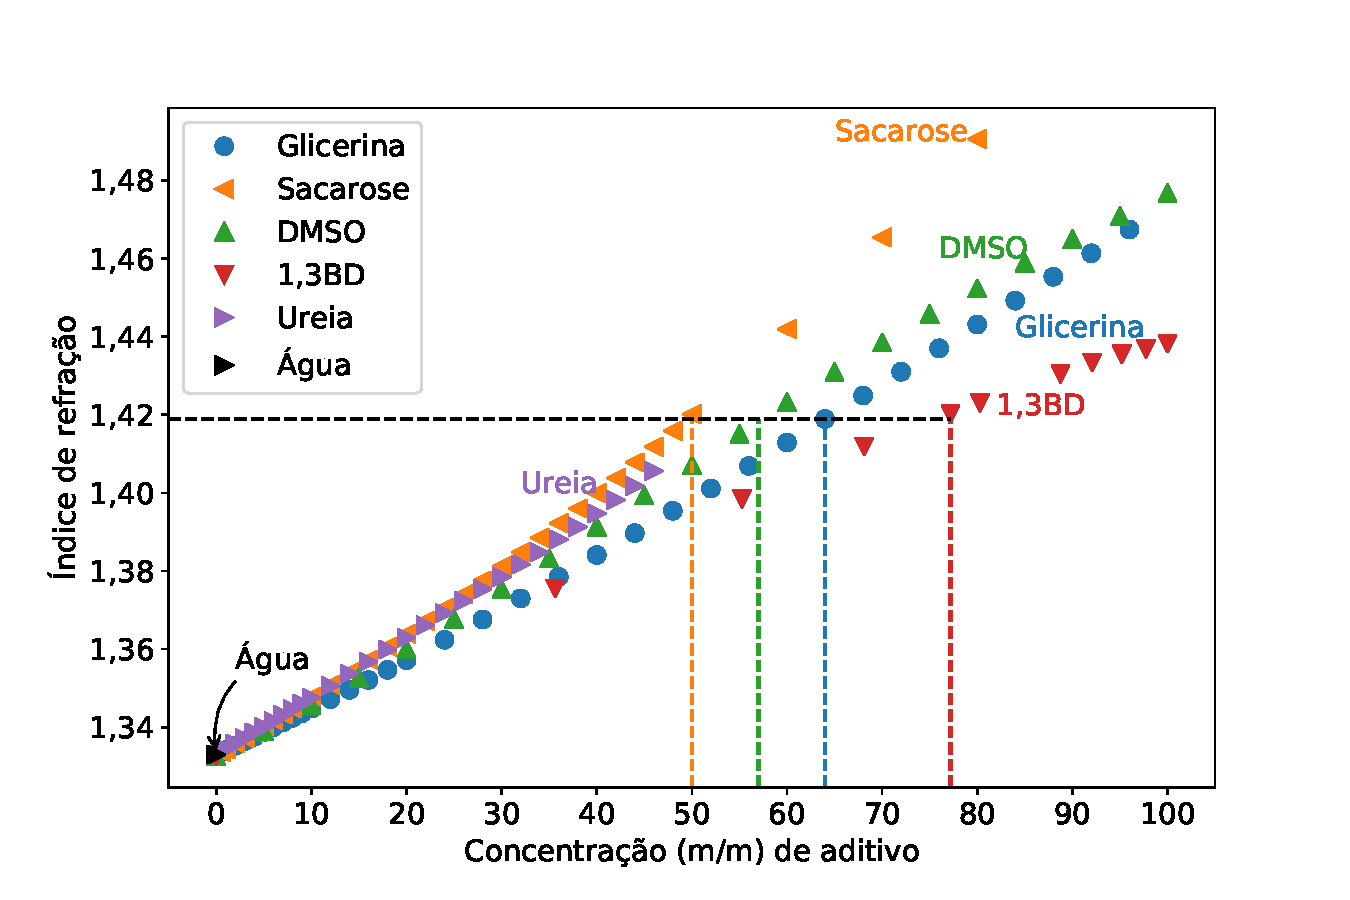
\includegraphics[width=0.7\textwidth]{imagens/propriedades/indice_refracao}
				\caption{Índice de refração em função da concentração de aditivo}
				\label{fig:indice_refracao}
			\end{figure}
	
			Inicialmente, comparou-se o sistema melhor estudado (glicerina) com sacarose, escolhida pois também possuía efeitos semelhantes à glicerina no intumescimento lamelar. A figura \ref{fig:rh_sacarose_glicerina} mostra os diagramas de viscosidade para soluções de micelas gigantes com 100 \mM{} de \CTAB, em concentrações crescentes de glicerina, e no ponto de igualdade no índice de refração de sacarose, 50\%.
			
			\begin{figure}[h]
				\centering
				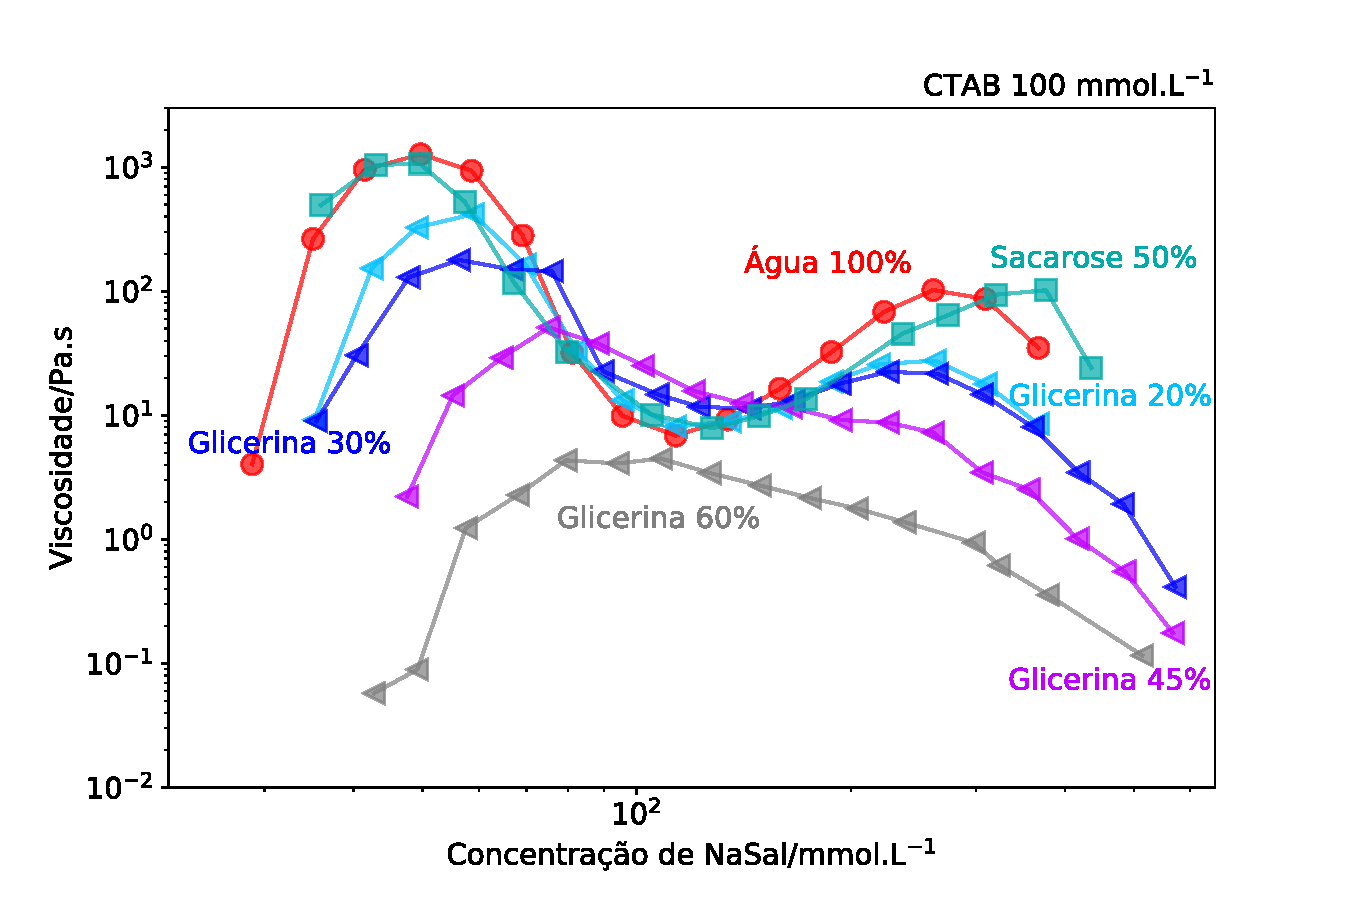
\includegraphics[width=0.7\textwidth]{imagens/reologia/RH_sacarose_glicerina}
				\caption{Viscosidade no repouso \(\eta_0\) em função da concentração de salicilato de sódio (NaSal) em várias concentrações dos aditivos glicerina e sacarose. 60\% de glicerina (V/V) e 50\% de sacarose (m/m) estão no ponto de equivalência do índice de refração.}
				\label{fig:rh_sacarose_glicerina}
			\end{figure} % todo: mencionar que curvas a laila mediu. Foram as de glicerina?
			
			Podemos observar que os dois picos de viscosidade observados em pequenas concentrações de glicerina, diminuem, e a região central permanece pouco afetada, como já havia sido descrito por Hoffmann. Porém, vemos que a adição de 50\% de sacarose praticamente não afetou a viscosidade das soluções, apesar da igualdade no índice de refração dessas soluções. Isso mostra que considerar somente o índice de refração não permite a previsão do comportamento dessas soluções, e isso motivou a realização de estudos posteriores.
			
			A figura \ref{fig:rh_13bd_dmso} mostra como os aditivos 1,3-butanodiol e dimetilsulfóxido afetam o perfil de viscosidade.
			
			\begin{figure}[h]
				\centering
				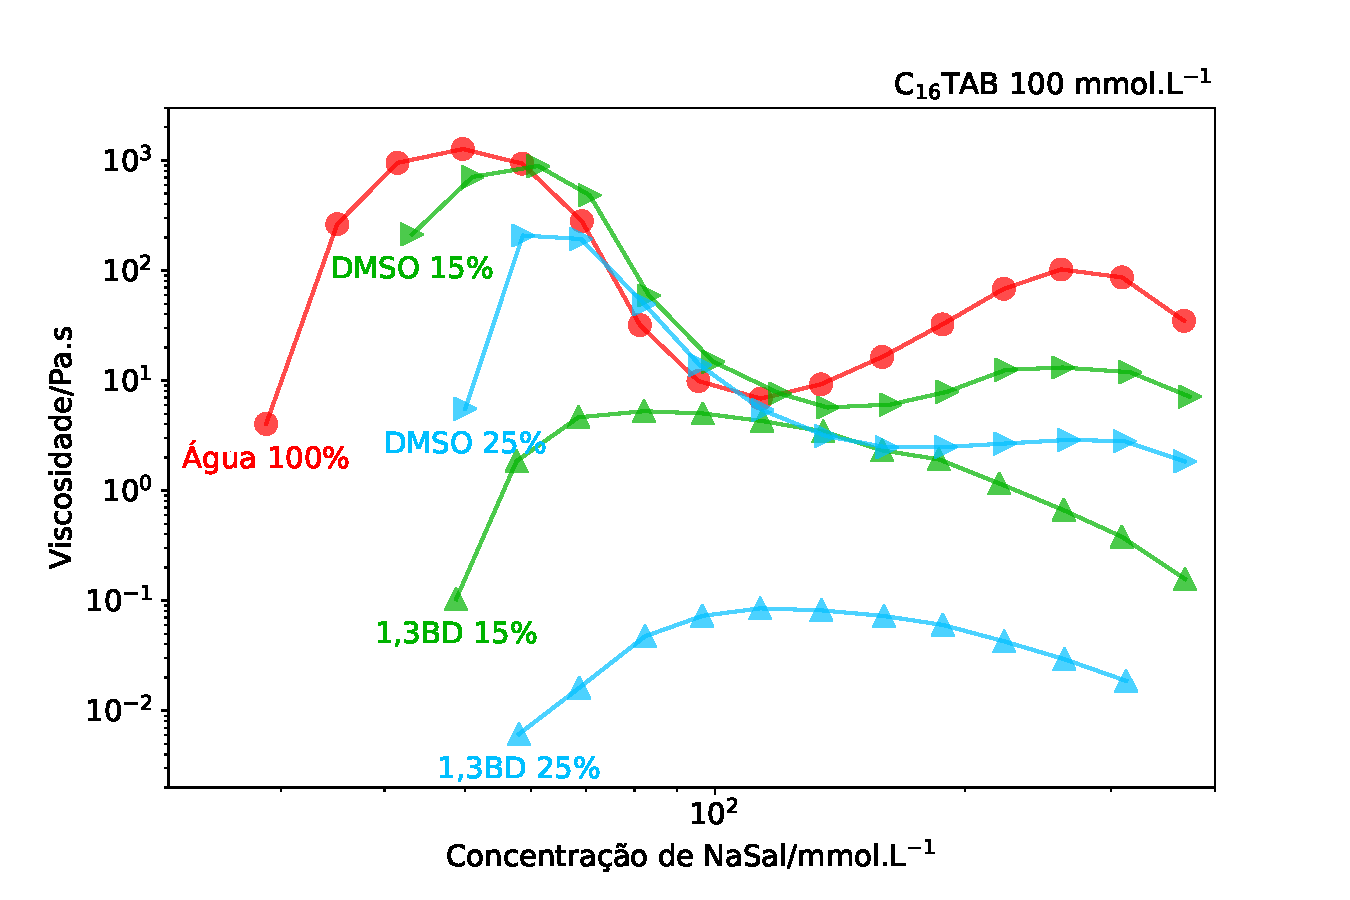
\includegraphics[width=0.7\textwidth]{imagens/reologia/RH_13BD_DMSO}
				\caption{Viscosidade no repouso \(\eta_0\) em função da concentração de salicilato de sódio (NaSal) em várias concentrações dos aditivos 1,3-butanodiol (1,3BD) e dimetilsulfóxido (DMSO). As concentrações de igualdade do índice de refração são 77\% (m/m) e 57\% (m/m), respectivamente}
				\label{fig:rh_13bd_dmso}
			\end{figure}
		
			O perfil de viscosidade dessas soluções foi muito mais afetado pelos aditivos do que era esperado observando-se somente o índice de refração, em especial o 1,3-butanodiol, onde 15\% (m/m) possui o mesmo efeito na viscosidade que 60\% de glicerina.
			
			A ureia possui o comportamento que mais difere dos outros aditivos, como mostra a figura \ref{fig:rh_ureia}.
			
			\begin{figure}[h]
				\centering
				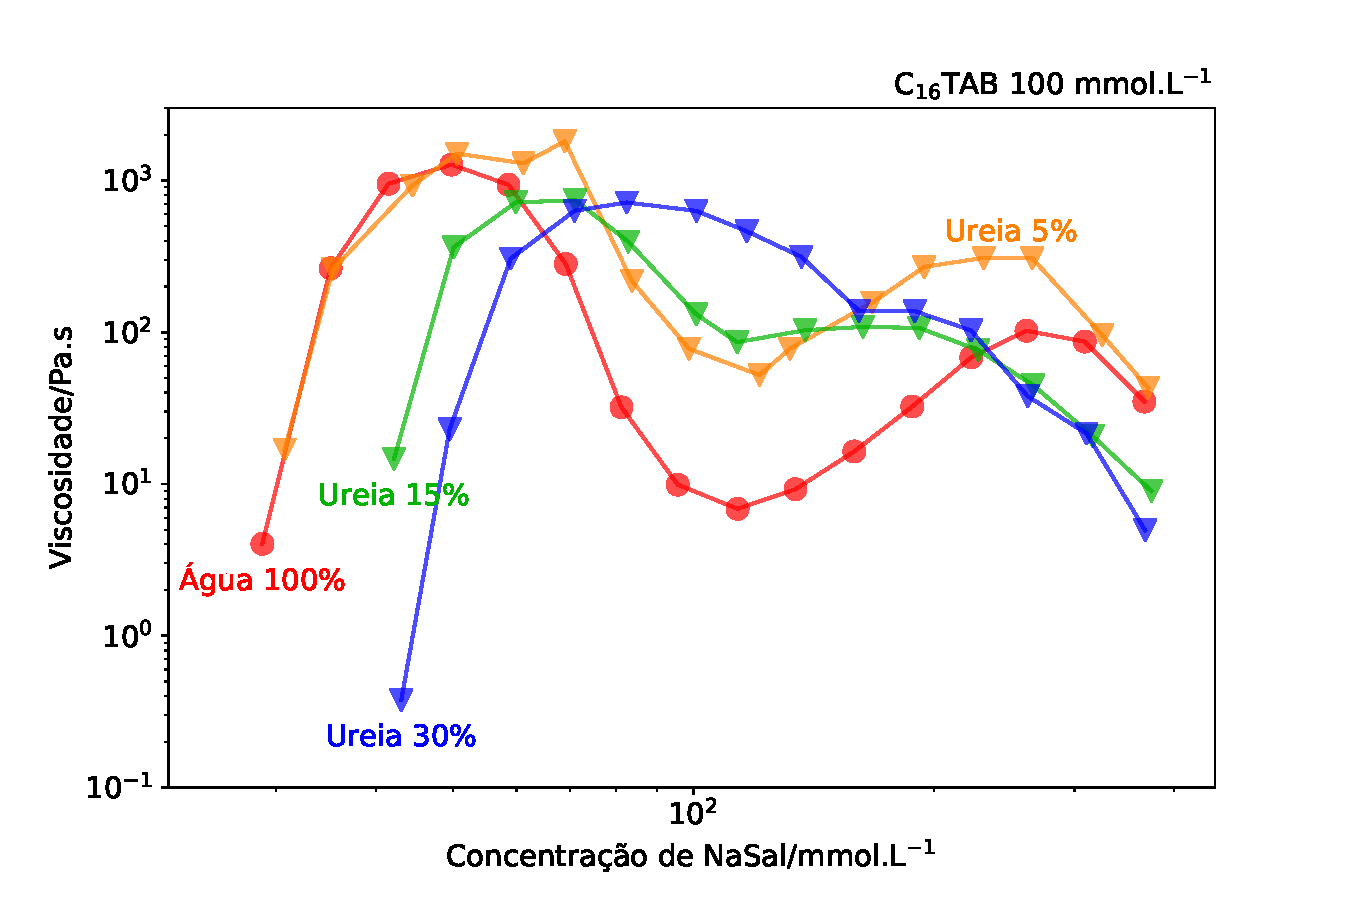
\includegraphics[width=0.7\textwidth]{imagens/reologia/RH_ureia}
				\caption{Viscosidade no repouso \(\eta_0\) em função da concentração de salicilato de sódio (NaSal) em várias concentrações de ureia. A concentração de igualdade de índice de refração é em torno de 55\%.}
				\label{fig:rh_ureia}
			\end{figure}

			Nesse caso, a viscosidade na região central aumentou, algo não observado nos outros cossolutos. Outro caso que possui um comportamento semelhante é o diagrama de orto-hidróxicinamato e \CTAB{} em pH 9. %todo: citar o artigo do OHCA
		
		\FloatBarrier
		
		\section{Efeito dos aditivos na calorimetria de micelas gigantes}
		
			A calorimetria de titulação isotérmica fornece informações sobre o quão favorável é a formação das micelas, através da concentração de formação de micelas gigantes, \cwlm. As figuras \ref{fig:itc_mg_glicerina} -- \ref{fig:itc_mg_ureia} mostram os perfis de formação de micelas gigantes para glicerina, sacarose, 1,3-butanodiol, dimetilsulfóxido e ureia.
		
			\begin{figure}[h]
				\centering
				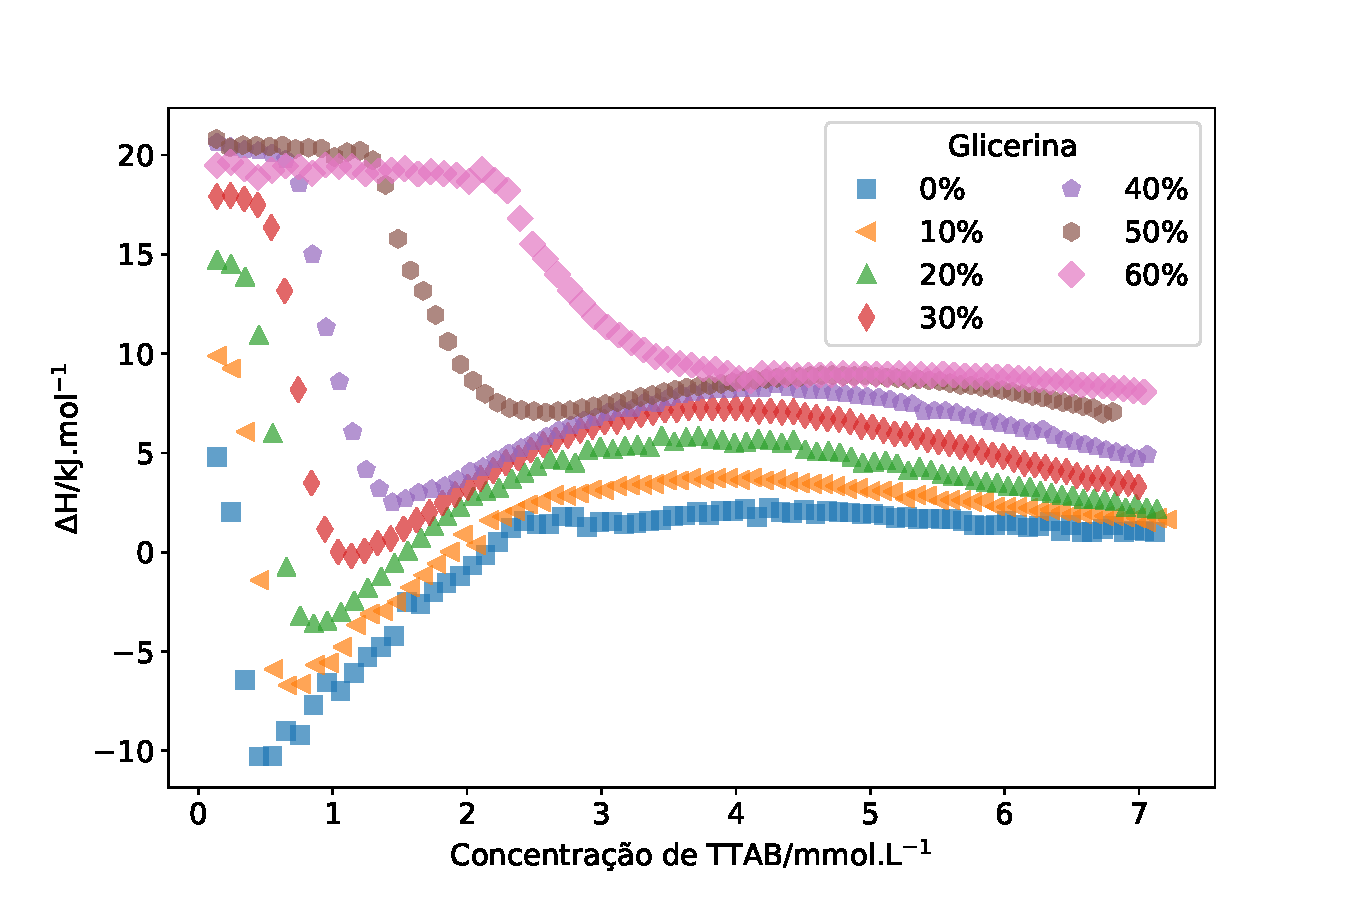
\includegraphics[width=0.7\textwidth]{imagens/itc/ITC_MG_glic}
				\caption{Efeito da concentração de glicerina nas curvas de titulação de formação de micelas gigantes. A concentração de salicilato de sódio na cela de amostra é de 1,5\mM. A concentração do aditivo está em \% (V/V).}
				\label{fig:itc_mg_glicerina}
			\end{figure}  % todo: colocar a curva sem aditivo em todos. Trocar o 0% por uma curva preta.
			
			\begin{figure}[h]
				\centering
				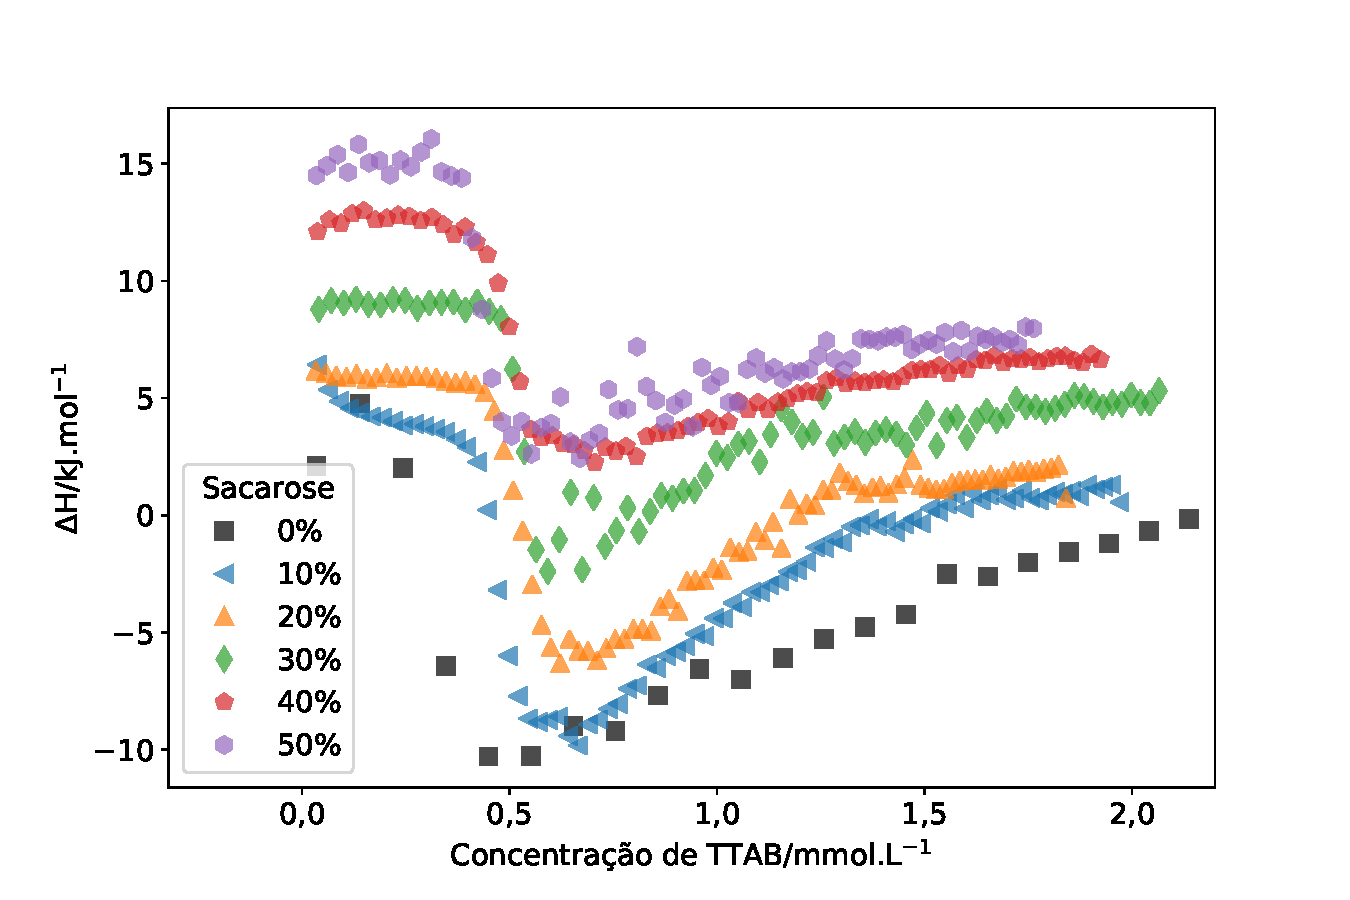
\includegraphics[width=0.7\textwidth]{imagens/itc/ITC_MG_sac}
				\caption{Efeito da concentração de sacarose nas curvas de titulação de formação de micelas gigantes. A concentração de salicilato de sódio na cela de amostra é de 1,5\mM. A concentração do aditivo está em \% (m/m).}
				\label{fig:itc_mg_sacarose}
			\end{figure}
			
			As diferenças entre glicerina e sacarose, novamente, se evidenciaram. Da mesma maneira que na reologia, a presença de sacarose não afetou a formação de micelas gigantes. Já a glicerina teve um efeito deletério, aumentando significativamente a concentração necessária para o crescimento.
						
			\begin{figure}[h]
				\centering
				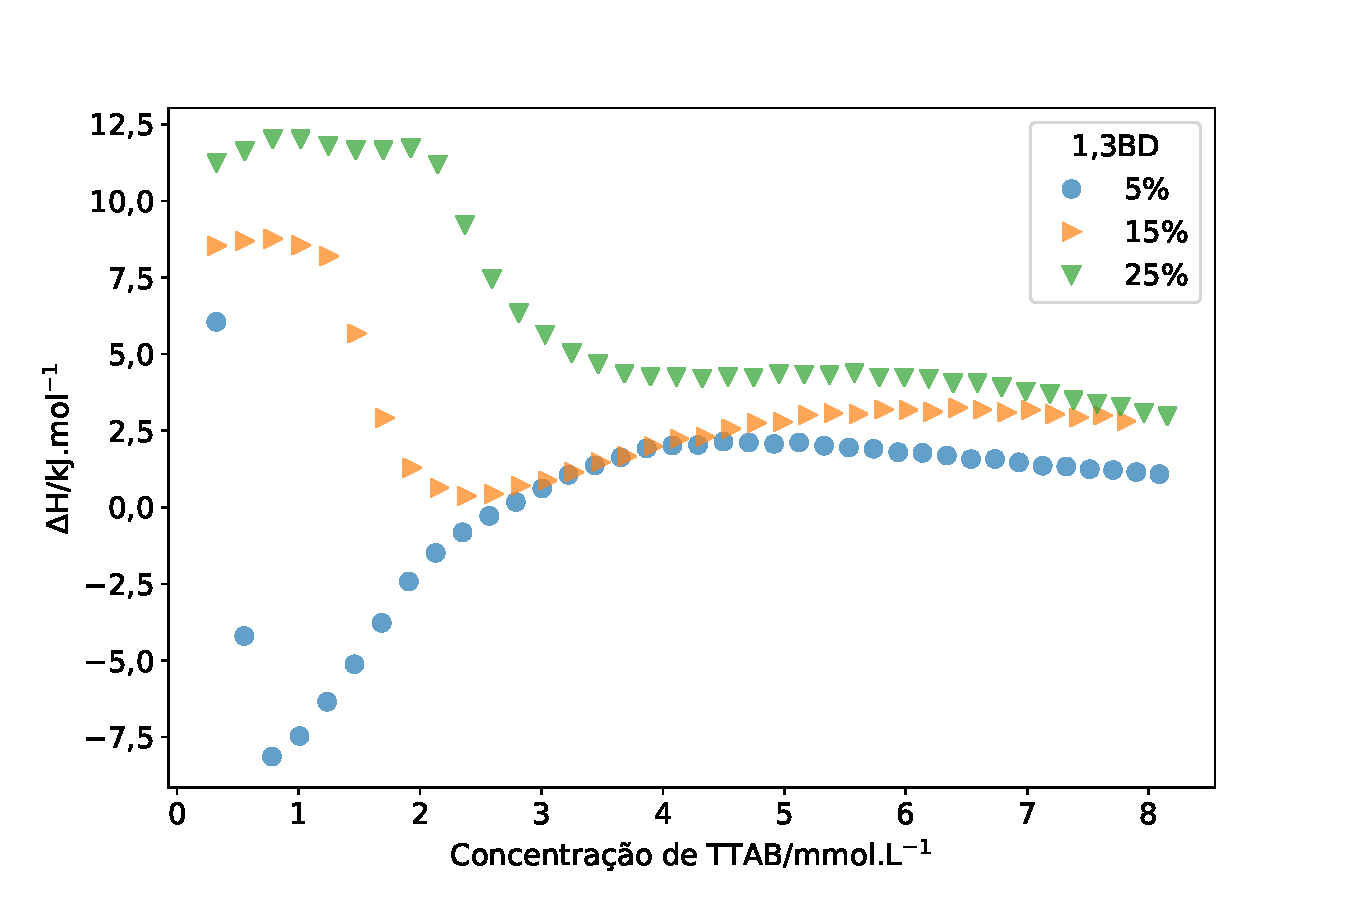
\includegraphics[width=0.7\textwidth]{imagens/itc/ITC_MG_13BD}
				\caption{Efeito da concentração de 1,3-butanodiol nas curvas de titulação de formação de micelas gigantes. A concentração de salicilato de sódio na cela de amostra é de 1,5\mM. A concentração do aditivo está em \% (m/m).}
				\label{fig:itc_mg_13bd}
			\end{figure}
			
			\begin{figure}[h]
				\centering
				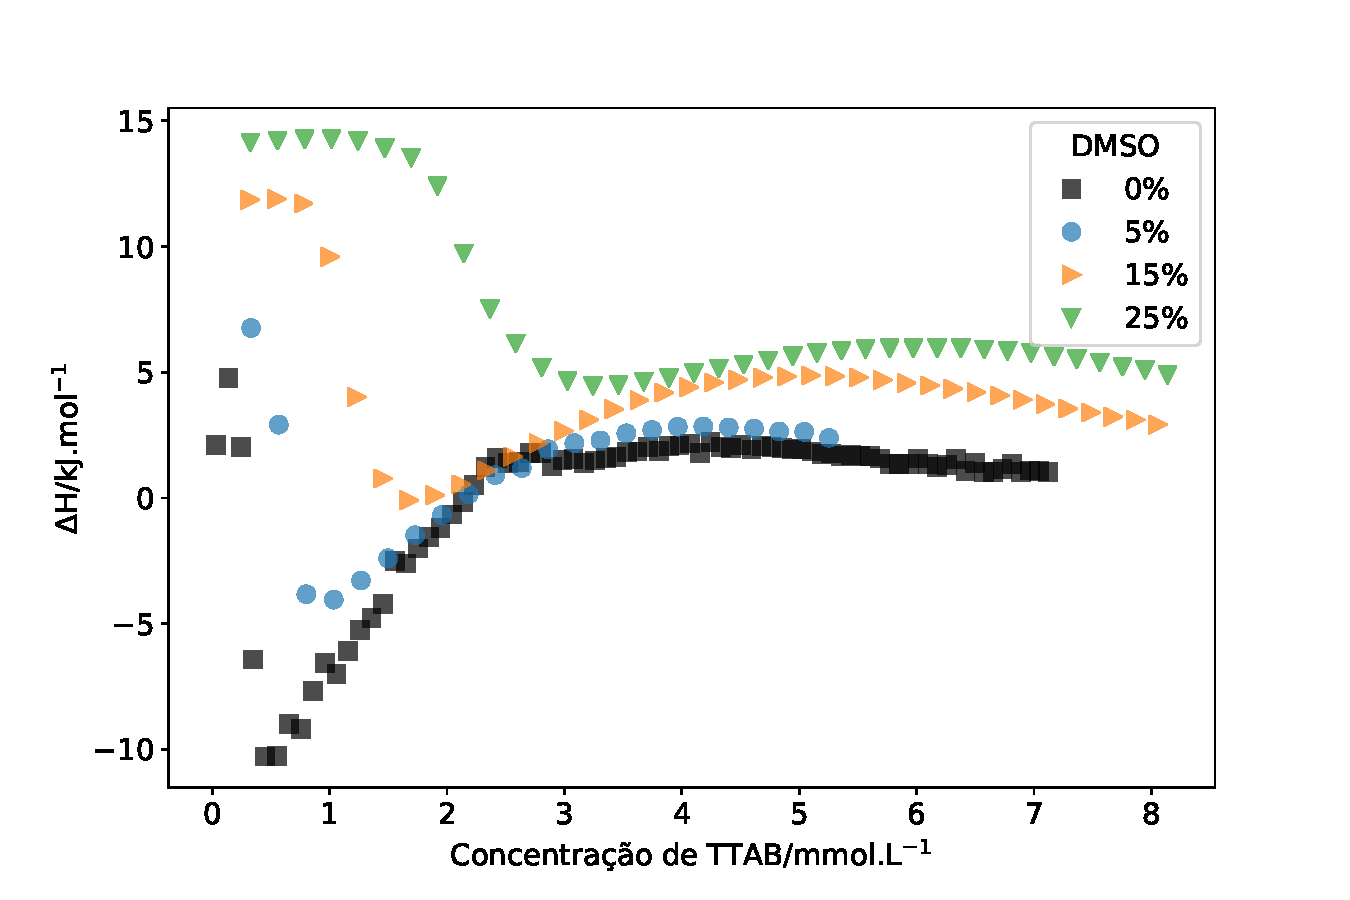
\includegraphics[width=0.7\textwidth]{imagens/itc/ITC_MG_dmso}
				\caption{Efeito da concentração de dimetilsulfóxido nas curvas de titulação de formação de micelas gigantes. A concentração de salicilato de sódio na cela de amostra é de 1,5\mM. A concentração do aditivo está em \% (m/m).}
				\label{fig:itc_mg_dmso}
			\end{figure}  % todo: será que dá pra juntar os dois?

			1,3-BD e DMSO não se mostraram muito diferentes, apesar dos perfis reológicos serem bastante distintos, algo não totalmente inesperado, já que ambas as técnicas observam fenômenos diferentes. Isso indica que a queda de viscosidade com 1,3-BD não se deve à uma desestabilização micelar, o que levaria à uma diminuição na quantidade de micelas.

			\begin{figure}[h]
				\centering
				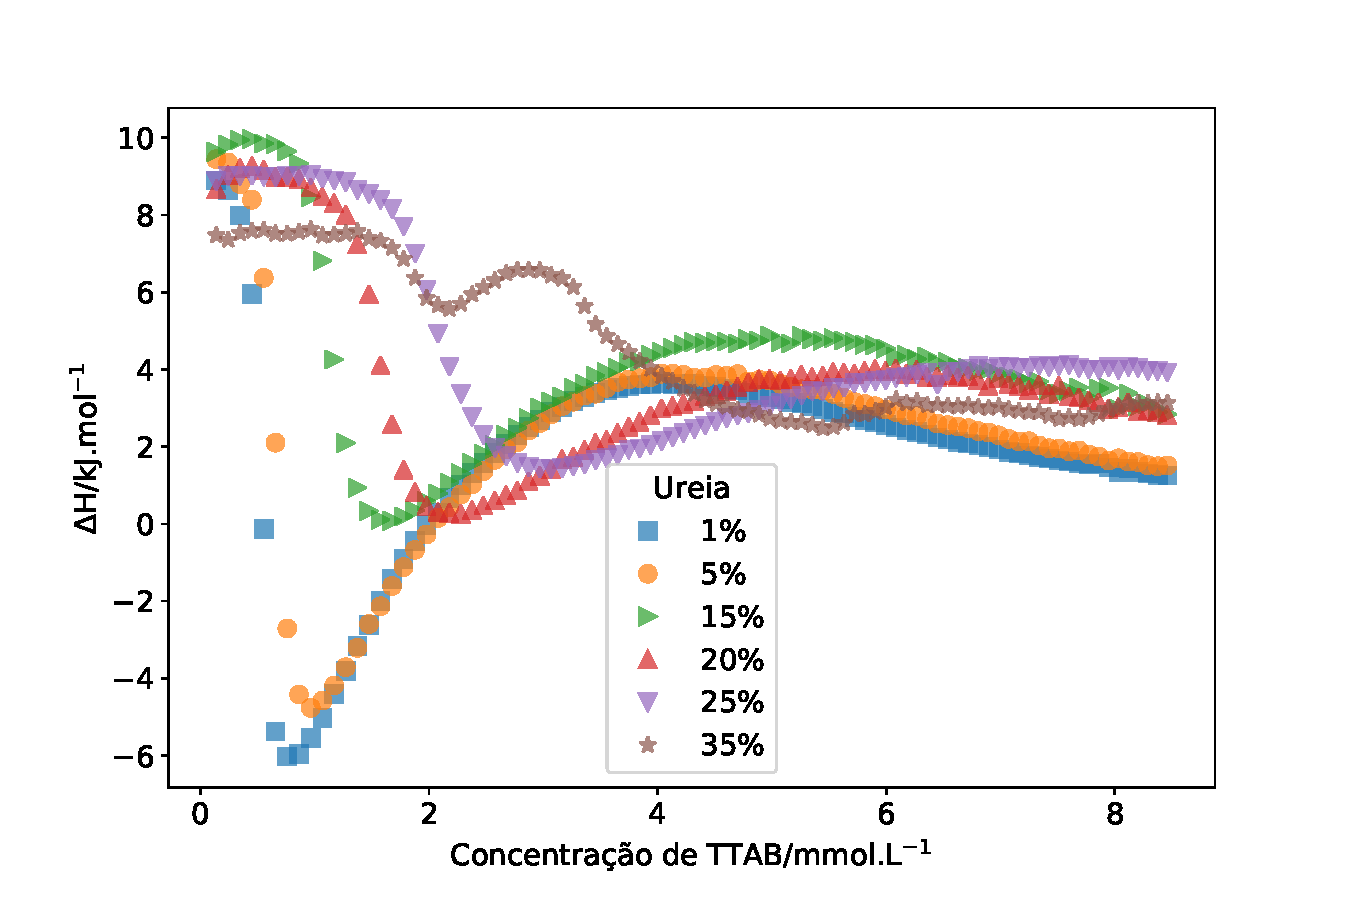
\includegraphics[width=0.7\textwidth]{imagens/itc/ITC_MG_ur}
				\caption{Efeito da concentração de ureia nas curvas de titulação de formação de micelas gigantes. A concentração de salicilato de sódio na cela de amostra é de 1,5\mM. A concentração do aditivo está em \% (m/m).}
				\label{fig:itc_mg_ureia}
			\end{figure}
		
			O comportamento da ureia seguiu o esperado, de acordo com a literatura, com um aumento de \cwlm{}. É interessante notar que o \DHwlm{} diminui com o aumento da concentração de ureia, o que sugere uma diminuição na adsorção de salicilato nas micelas. Em 35\% de ureia observa-se um perfil bastante diferente dos outros, porém nessa situação, ocorre a formação de um precipitado, cuja natureza será discutida na seção \ref{sec:cap_efeito_ureia}.
			
			Uma maneira de se resumir as curvas calorimétricas é através da concentração de formação de micelas gigantes (\cwlm) e a entalpia de micelização (\DHwlm). Dessa forma, podemos analisar o comportamento de todos os aditivos mais facilmente. A figura \ref{fig:cwlm_dhwlm_por_aditivo} resume isso, mostrando como essas propriedades variam com os aditivos, separadamente. A figura \ref{fig:cwlm_dhwlm_por_conc} mostra o mesmo, porém em função da concentração de aditivo.
			
			\begin{figure}[h]
				\begin{subfigure}[t]{0.5\textwidth}
					\centering
					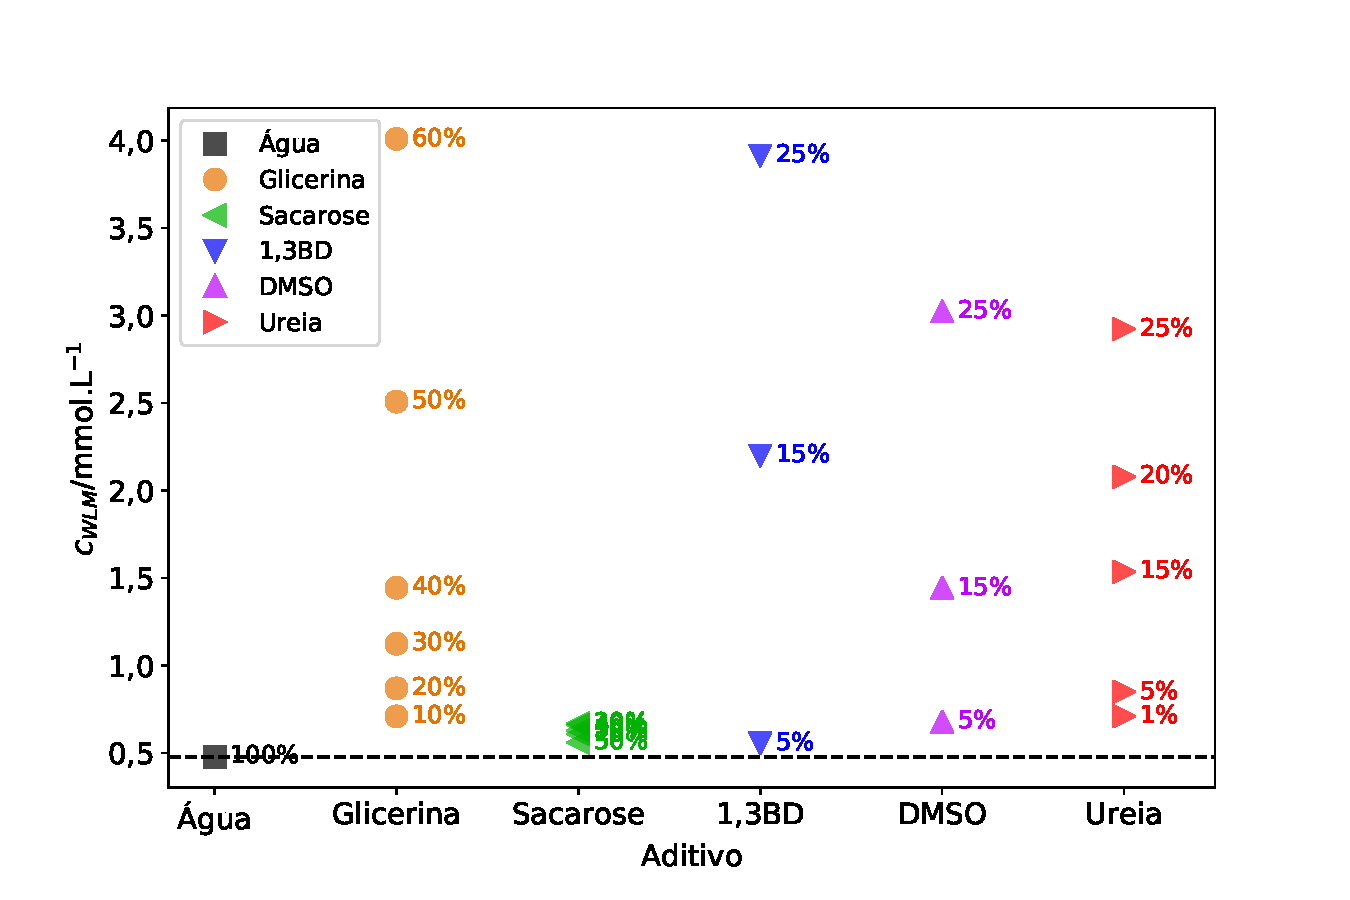
\includegraphics[width=\textwidth]{imagens/itc/Cwlm_por_Aditivo}
					\caption{\cwlm{}}
					\label{fig:cwlm_por_aditivo}
				\end{subfigure}%
				\begin{subfigure}[t]{0.5\textwidth}
					\centering
					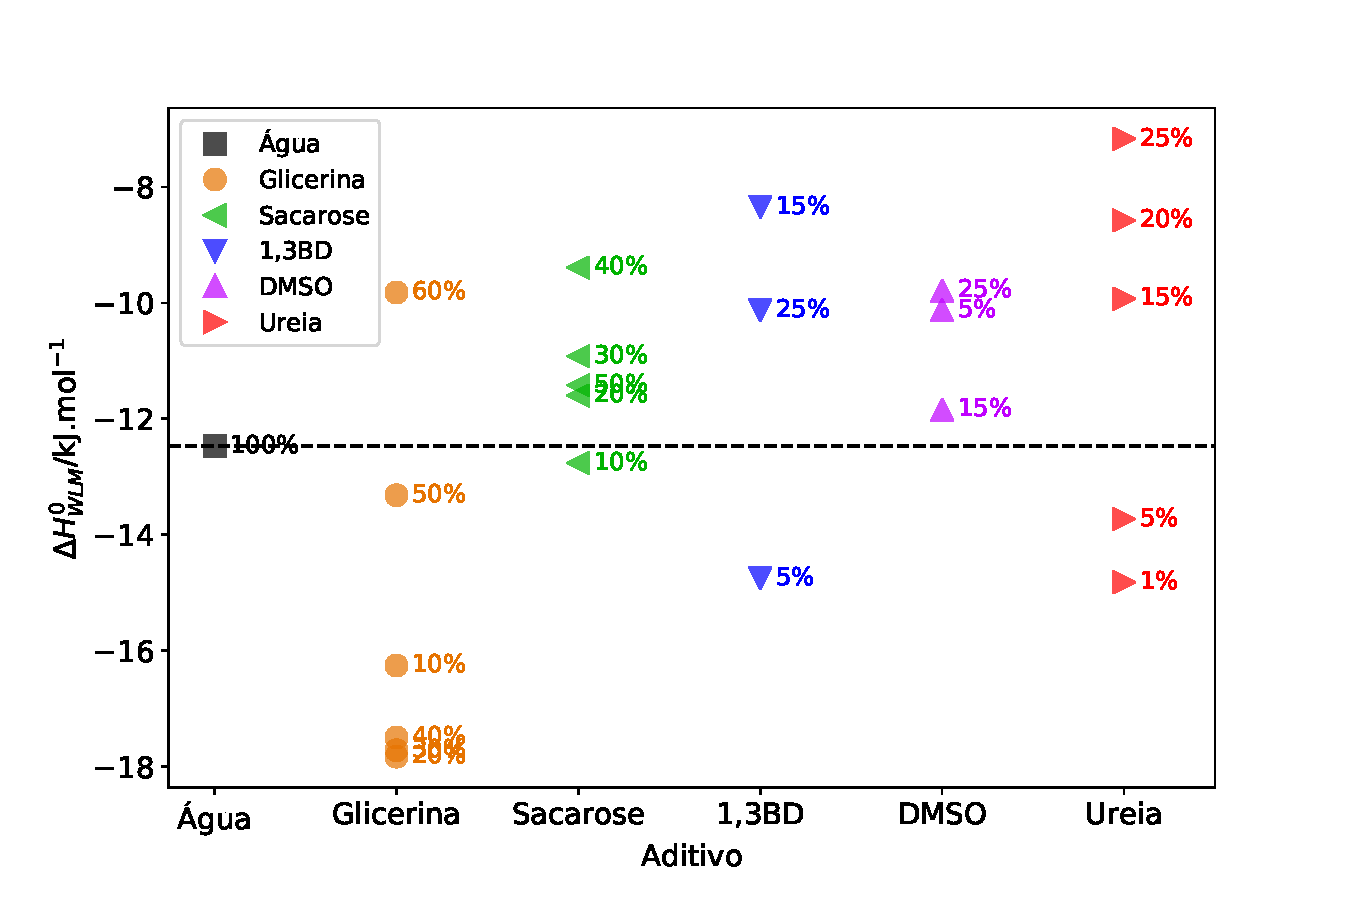
\includegraphics[width=\textwidth]{imagens/itc/DHwlm_por_Aditivo}
					\caption{\DHwlm{}}
					\label{fig:dhwlm_por_aditivo}
				\end{subfigure}
				\caption{\cwlm{} e \DHwlm{} em função dos aditivos e de sua concentração}
				\label{fig:cwlm_dhwlm_por_aditivo}
			\end{figure} 
		
			\begin{figure}[h]
				\begin{subfigure}[t]{0.5\textwidth}
					\centering
					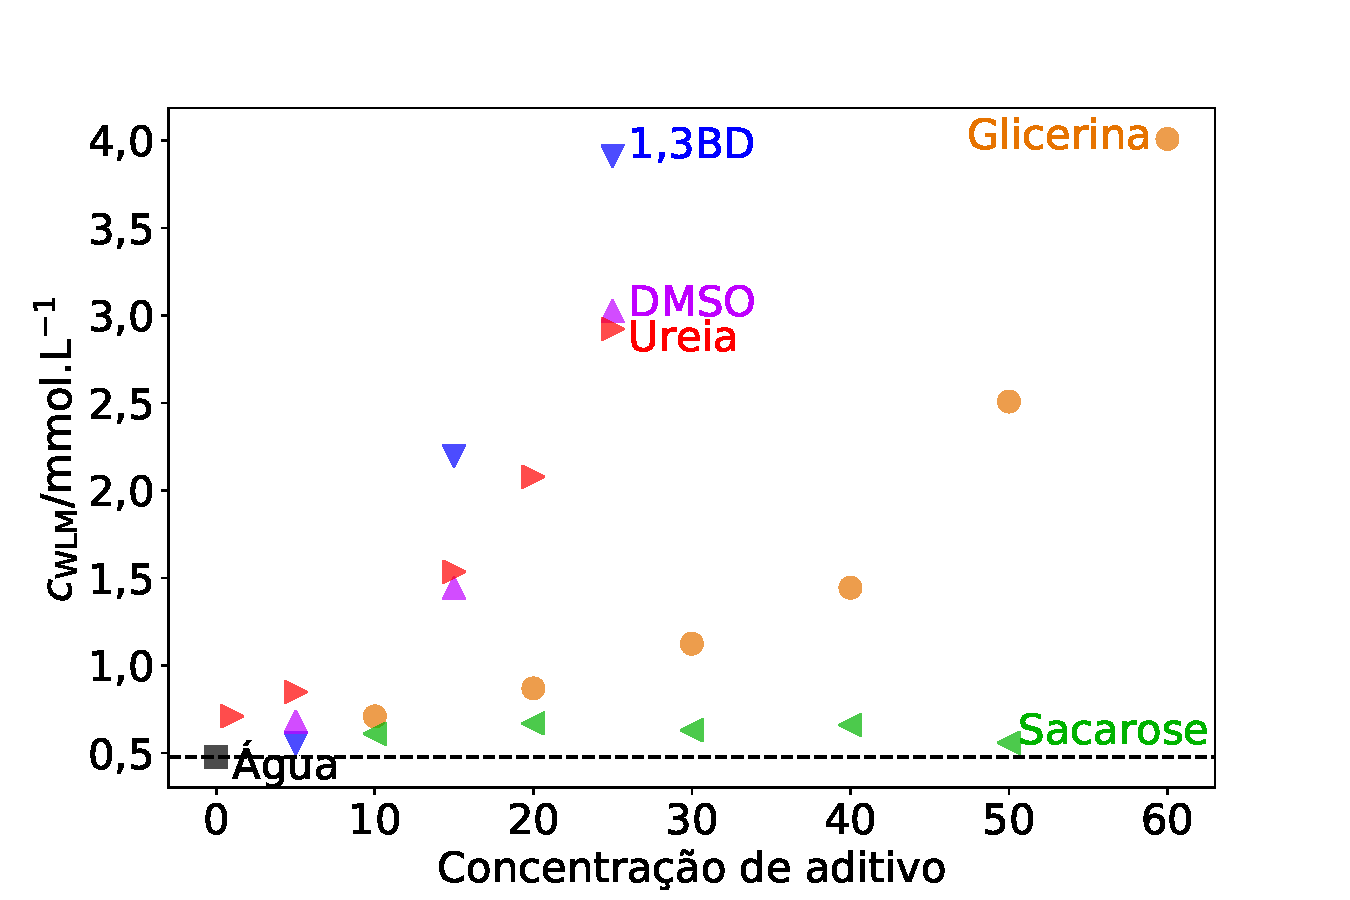
\includegraphics[width=\textwidth]{imagens/itc/Cwlm_por_conc}
					\caption{\cwlm}
					\label{fig:cwlm_por_conc}
				\end{subfigure} %
				\begin{subfigure}[t]{0.5\textwidth}
					\centering
					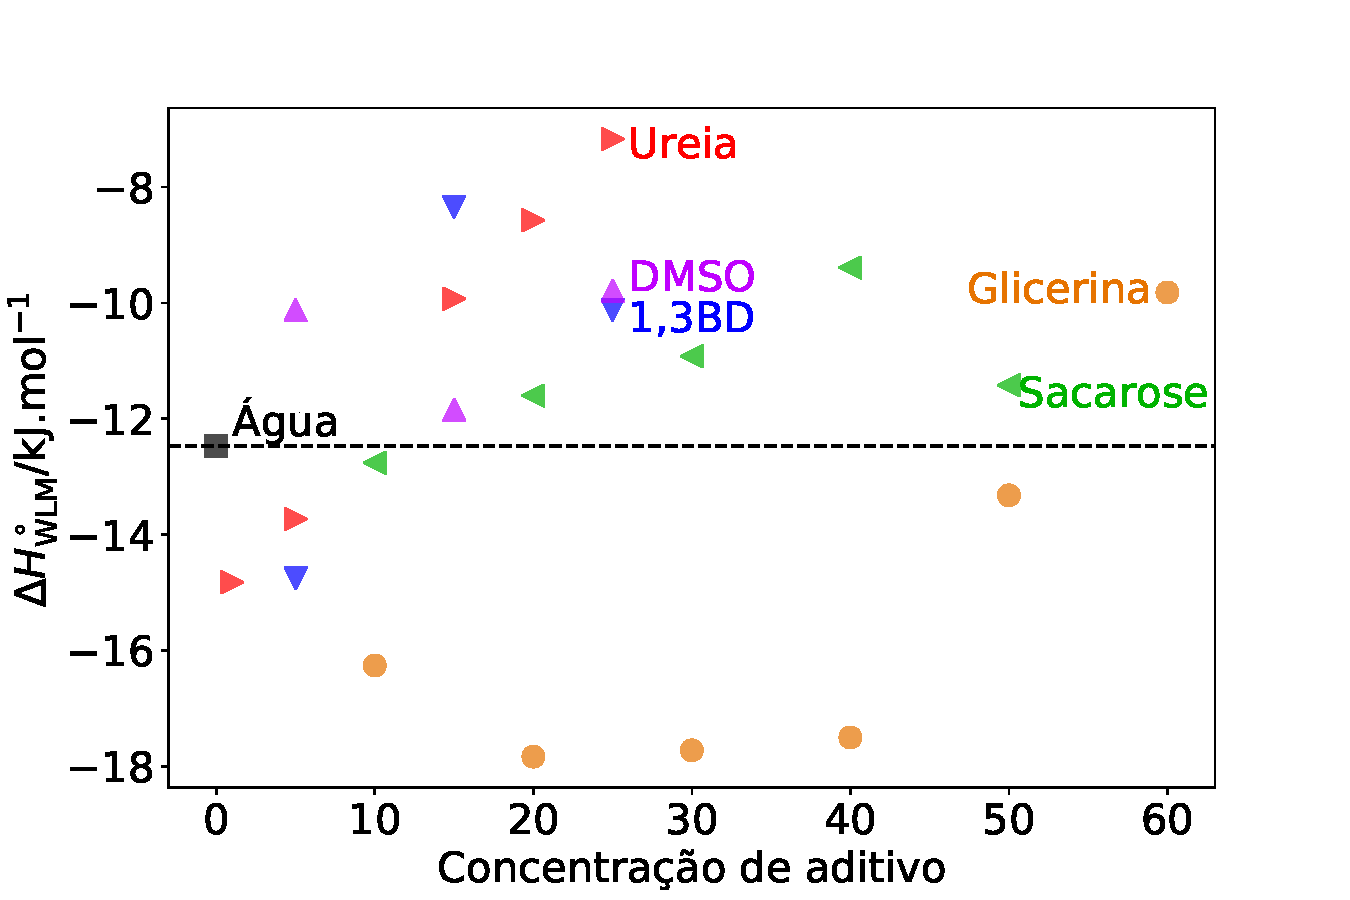
\includegraphics[width=\textwidth]{imagens/itc/DHwlm_por_conc}
					\caption{\DHwlm}
					\label{fig:dhwlm_por_conc}
				\end{subfigure}
				
				\caption{\cmc{} e \DHmic{} em função da concentração de aditivo.}
				\label{fig:cwlm_dhwlm_por_conc}
			\end{figure}
		
		\FloatBarrier
		
		\section{Efeito dos aditivos na calorimetria de micelização}
		
		A calorimetria de formação de micelas gigantes possui uma complexidade maior devido à presença do salicilato. Para facilitar a interpretação, foram obtidas informações da formação de micelas esféricas, titulando-se \TTAB{} em água. As figuras \ref{fig:itc_glicerina} -- \ref{fig:itc_ureia} mostram as curvas de titulação para glicerina, sacarose, 1,3-butanodiol, dimetilsulfóxido e ureia.
					
%			\begin{figure}[h]
%				\centering
%				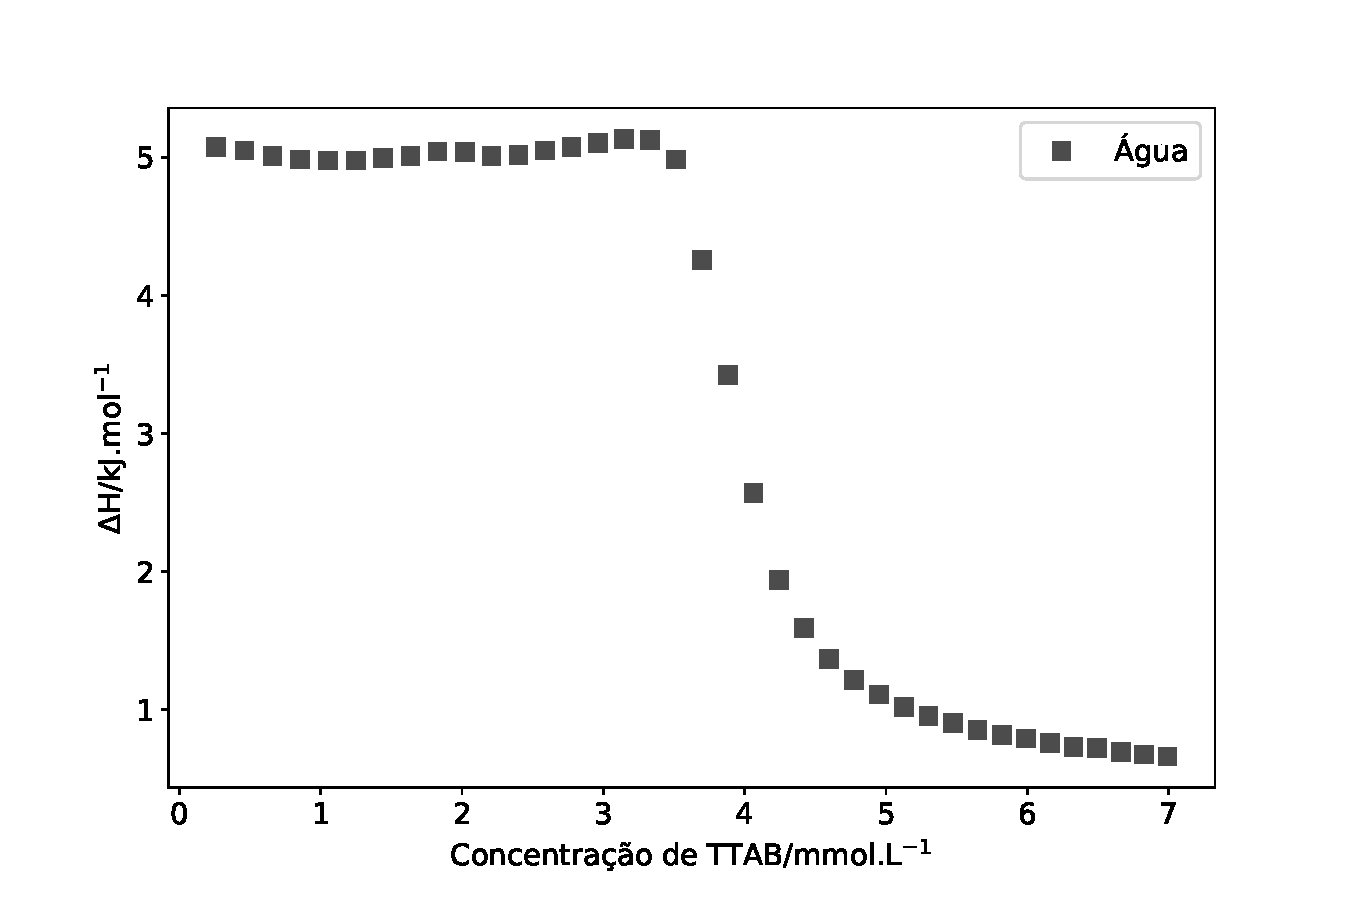
\includegraphics[width=0.7\textwidth]{imagens/itc/ITC_agua}
%				\caption{Titulação de \TTAB em água}
%				\label{fig:itc_agua}
%			\end{figure}
			
			\begin{figure}[h]
				\centering
				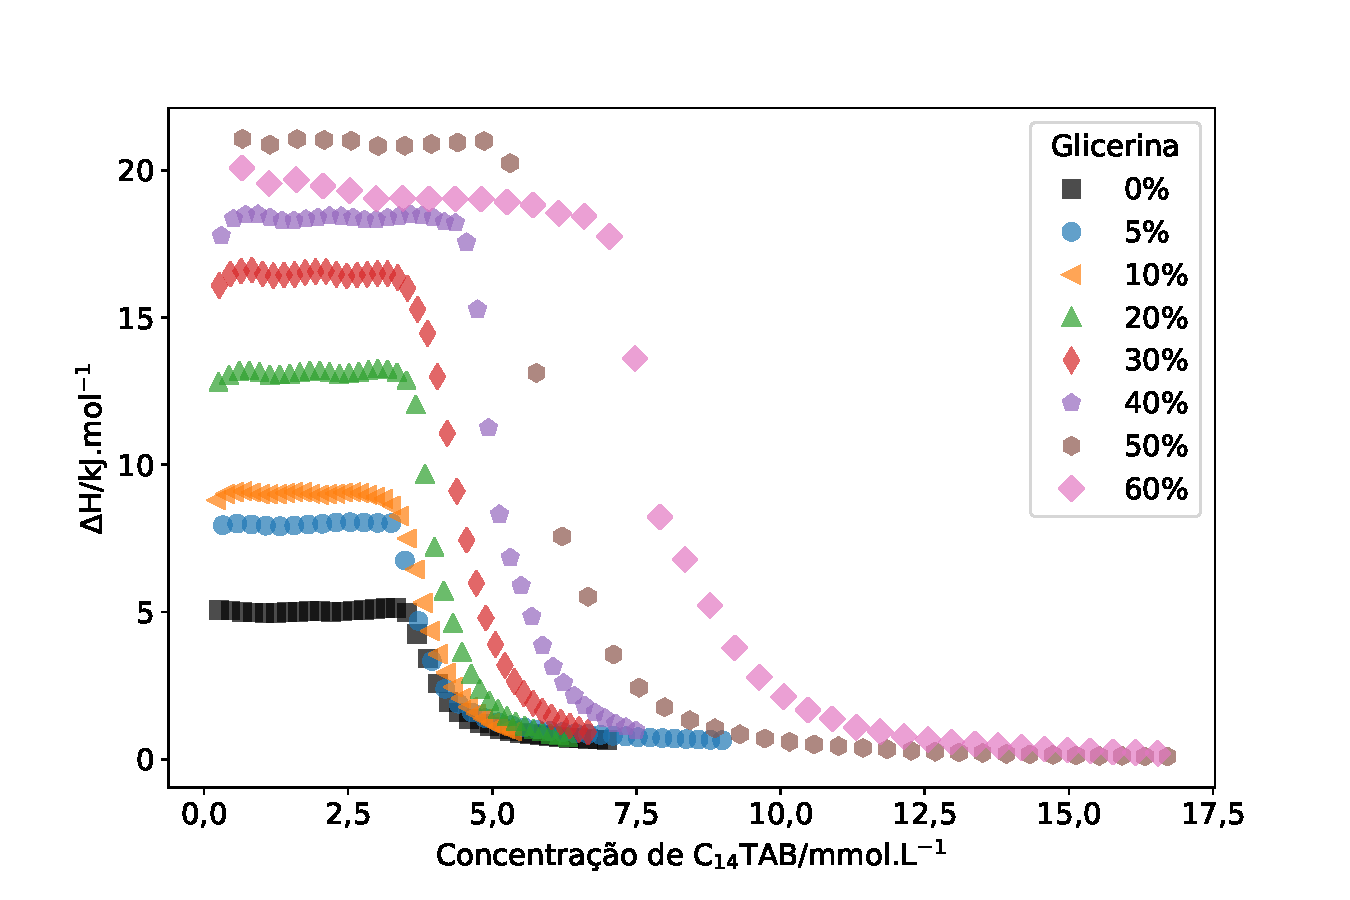
\includegraphics[width=0.7\textwidth]{imagens/itc/ITC_glic}
				\caption{Efeito da glicerina na titulação de \TTAB.}
				\label{fig:itc_glicerina}
			\end{figure}
		
			\begin{figure}[h]
				\centering
				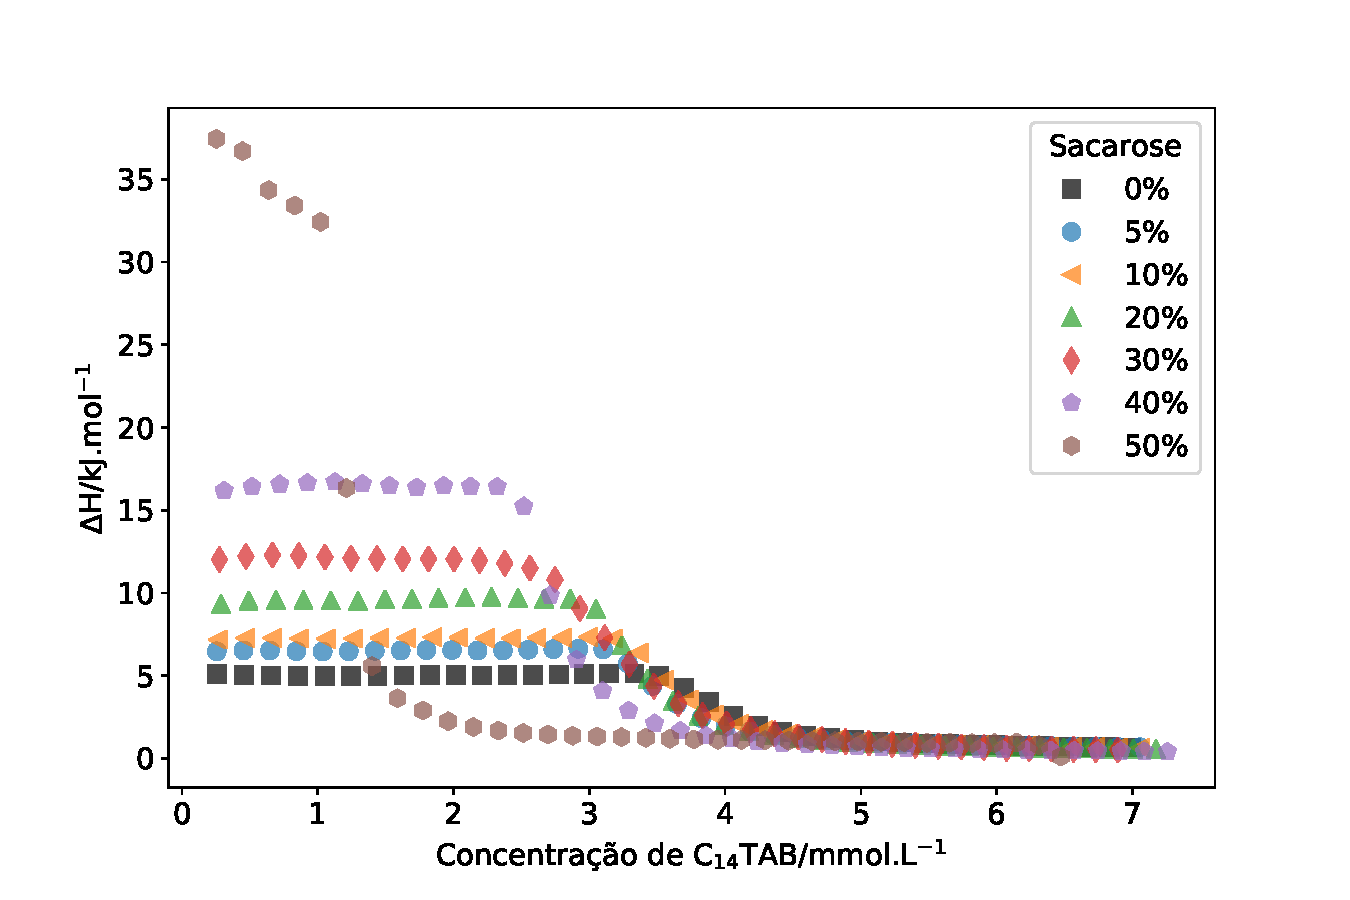
\includegraphics[width=0.7\textwidth]{imagens/itc/ITC_sac}
				\caption{Efeito de sacarose na titulação de \TTAB}
				\label{fig:itc_sacarose}
			\end{figure}
			
			O efeito da glicerina na formação de micelas é semelhante ao efeito em micelas gigantes, exceto pelo aumento do \DHmic{}. Mais interessante, porém, é que sacarose levou à uma diminuição da \cmc{}. Isso levanta duas perguntas. Em primeiro lugar, qual é o mecanismo de estabilização micelar, e depois, porque esse mecanismo não afeta a formação de micelas gigantes?
			
			% todo: ref
			A literatura aponta que os grupos hidroxila pode interagir com a superfície micelar, diminuindo a repulsão entre as cabeças, estabilizando as micelas. Porém, nas micelas gigantes, o grupo carboxilato do salicilato se encontra nessa mesma região, então há uma competição entre esses dois grupos. Como o carboxilato é carregado, interage mais fortemente com as micelas e impede que a sacarose exerça sua influência estabilizadora. 
			
			\begin{figure}[h]
				\centering
				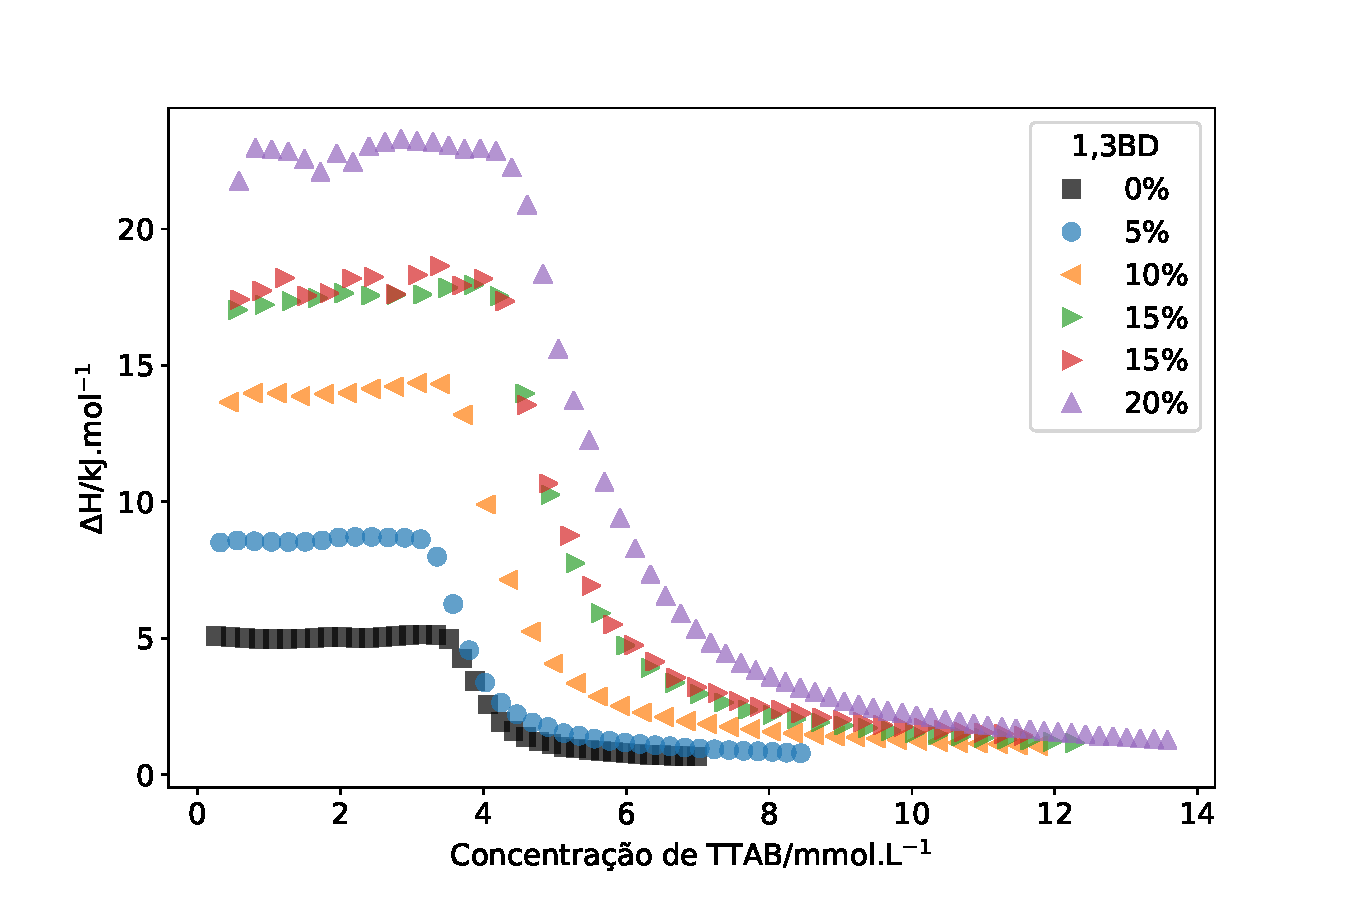
\includegraphics[width=0.7\textwidth]{imagens/itc/ITC_13BD}
				\caption{Efeito de 1,3-butanodiol na titulação de \TTAB}
				\label{fig:itc_13bd}
			\end{figure} 
		
			\begin{figure}[h]
				\centering
				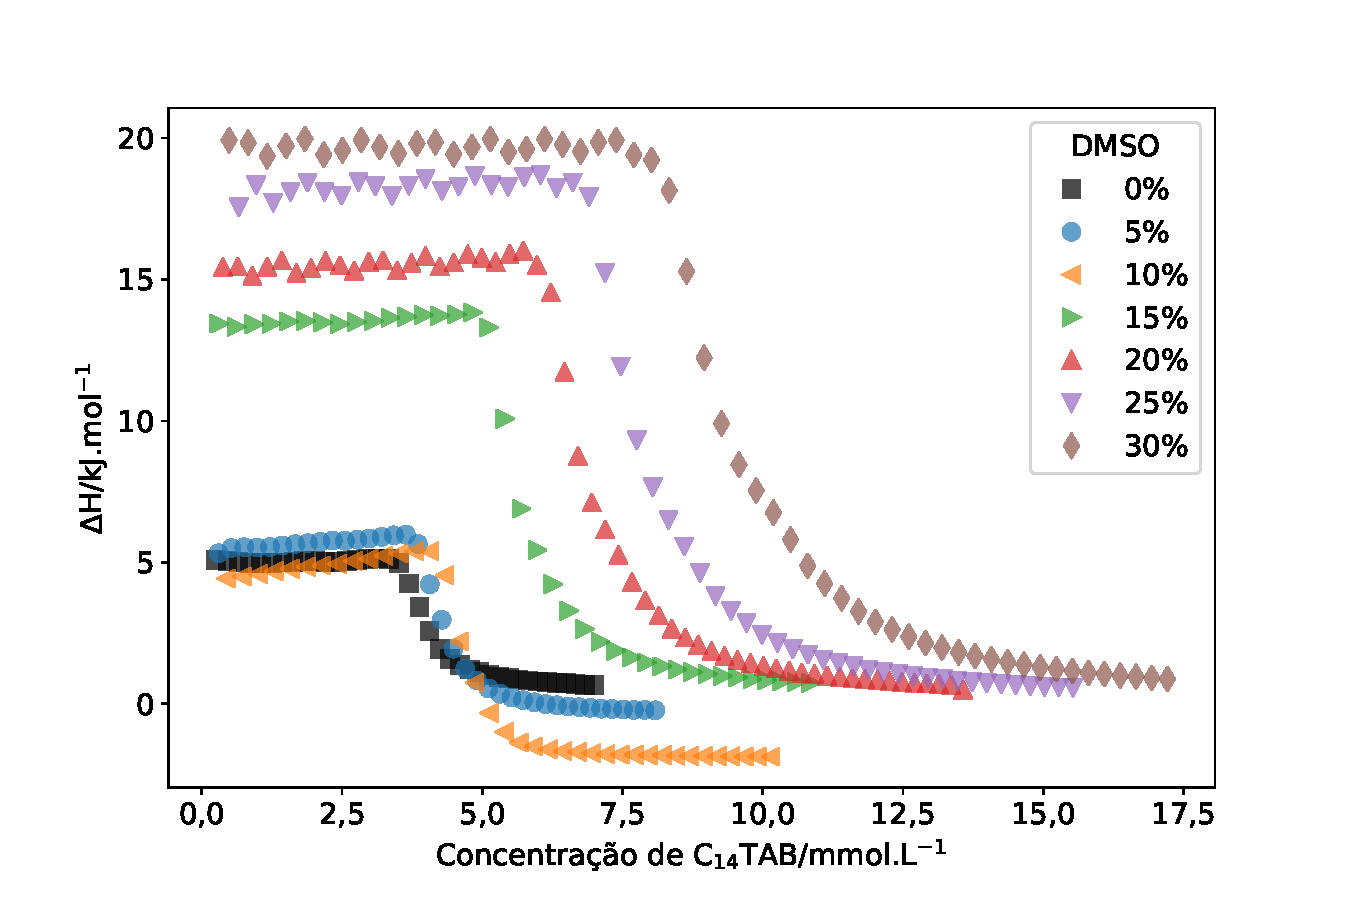
\includegraphics[width=0.7\textwidth]{imagens/itc/ITC_dmso}
				\caption{Efeito de dimetilsulfóxido na titulação de \TTAB.}
				\label{fig:itc_dmso}
			\end{figure}
			
			Novamente, o 1,3-BD e DMSO mostraram possuir comportamentos semelhantes entre si, portanto o mecanismo que influencia ambas as micelas gigantes quanto esféricas deve ser semelhante.
			
			\begin{figure}[h]
				\centering
				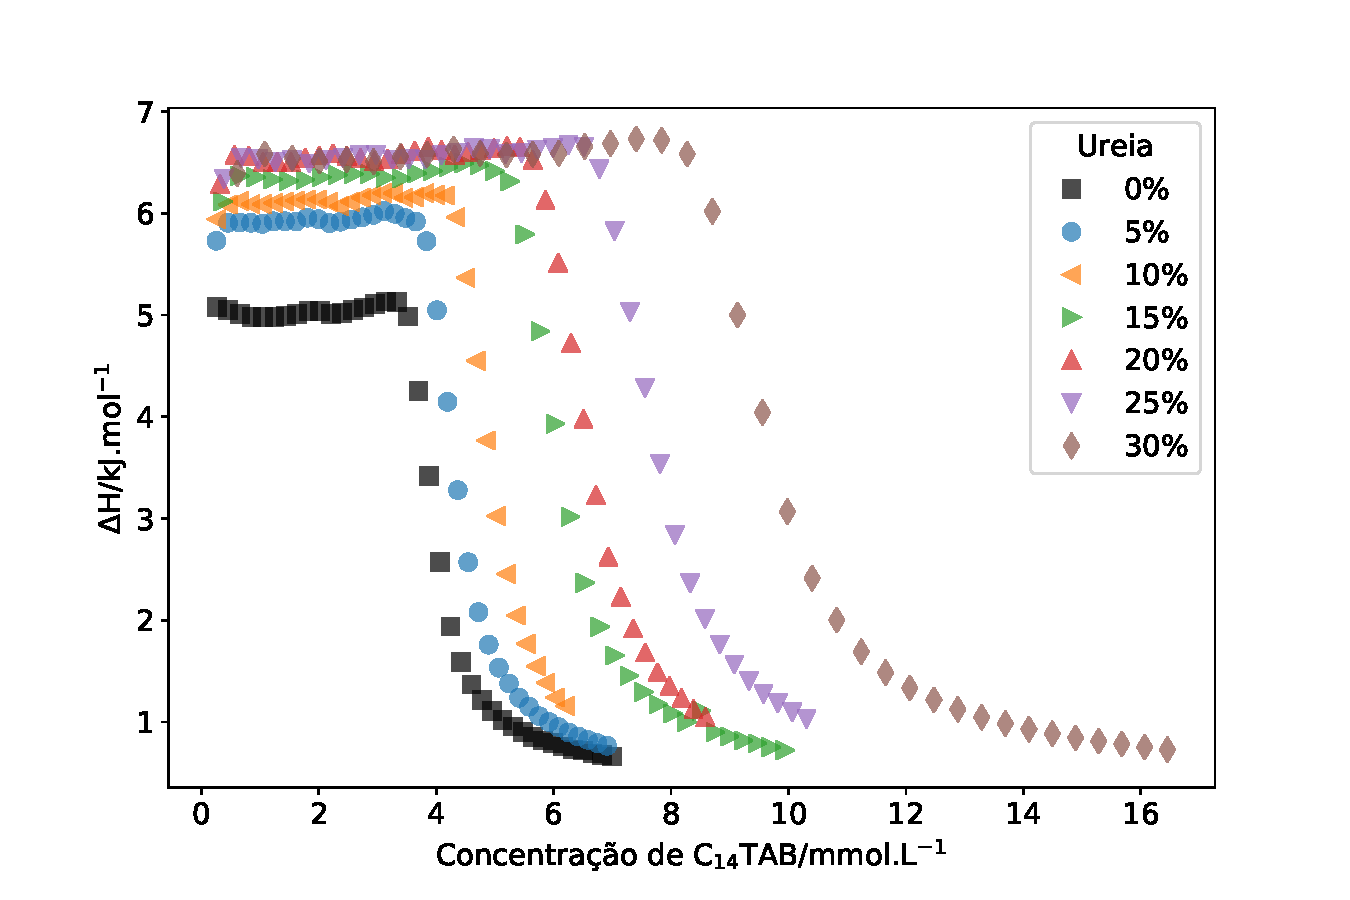
\includegraphics[width=0.7\textwidth]{imagens/itc/ITC_ur}
				\caption{Efeito de ureia na titulação de \TTAB.}
				\label{fig:itc_ureia}
			\end{figure}
		
		A ureia influencia aumentando a \cmc{}, como esperado, porém não afeta muito o \DHmic{}. Logo, como não há \Sal{} para ser dessorvido das micelas, devido à alta constante dielétrica do meio, não há variações de \DHmic.
		
		As concentrações micelares críticas (\cmc) e entalpias de micelização (\DHmic) foram utilizadas para resumir as informações desta seção. A figura \ref{fig:cmc_dh_por_composto} mostra como as propriedades são afetadas pelos vários aditivos e suas concentrações, separadamente, e a figura \ref{fig:cmc_dh_por_conc} faz o mesmo, porém em função da concentração de aditivo.
		
		\begin{figure}[h]
			\begin{subfigure}[t]{0.5\textwidth}
				\centering
				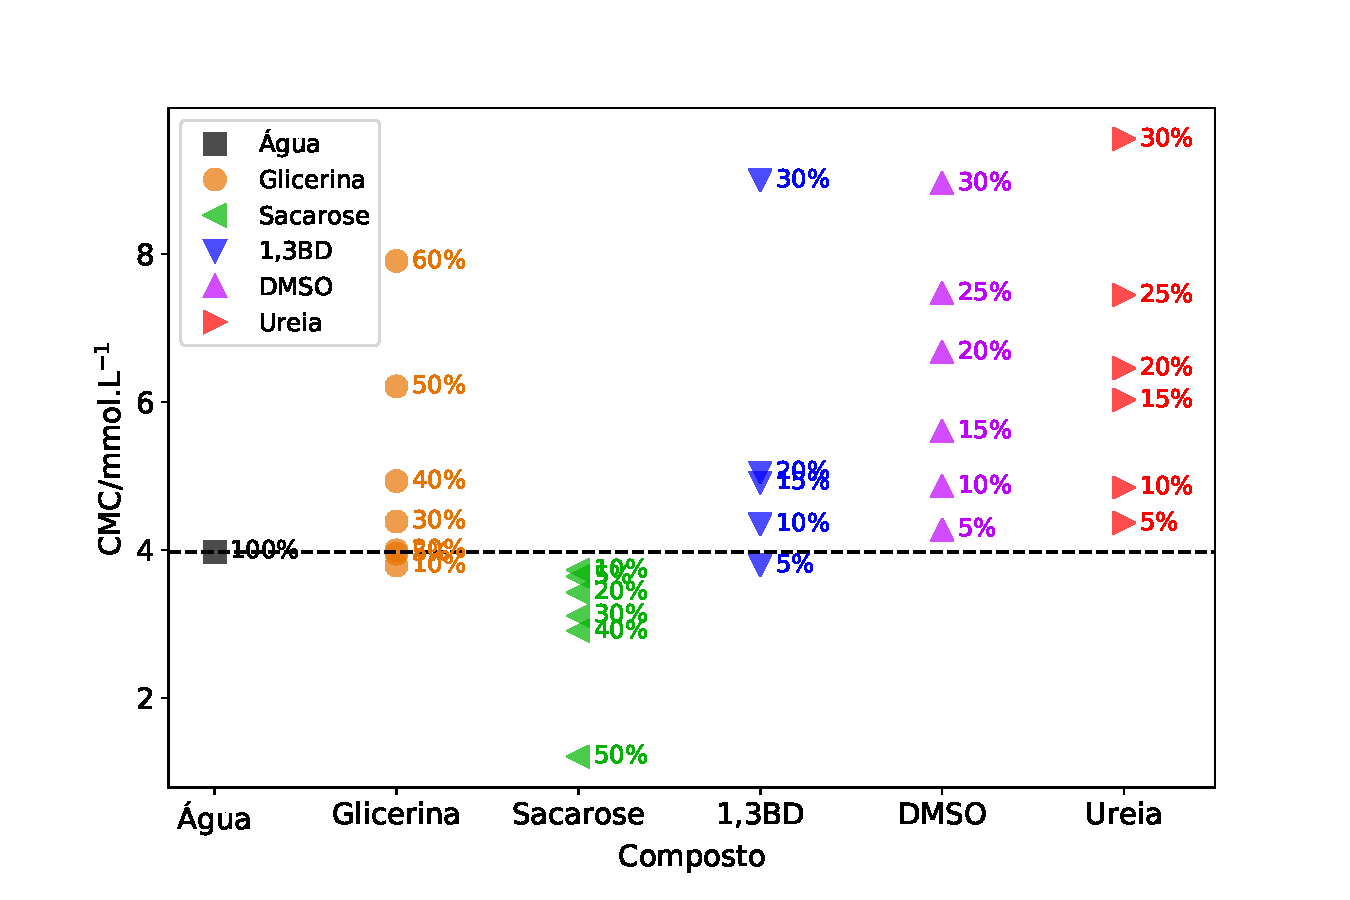
\includegraphics[width=\textwidth]{imagens/itc/CMC_por_composto}
				\caption{\cmc}
				\label{fig:cmc_por_composto}
			\end{subfigure} %
			\begin{subfigure}[t]{0.5\textwidth}
				\centering
				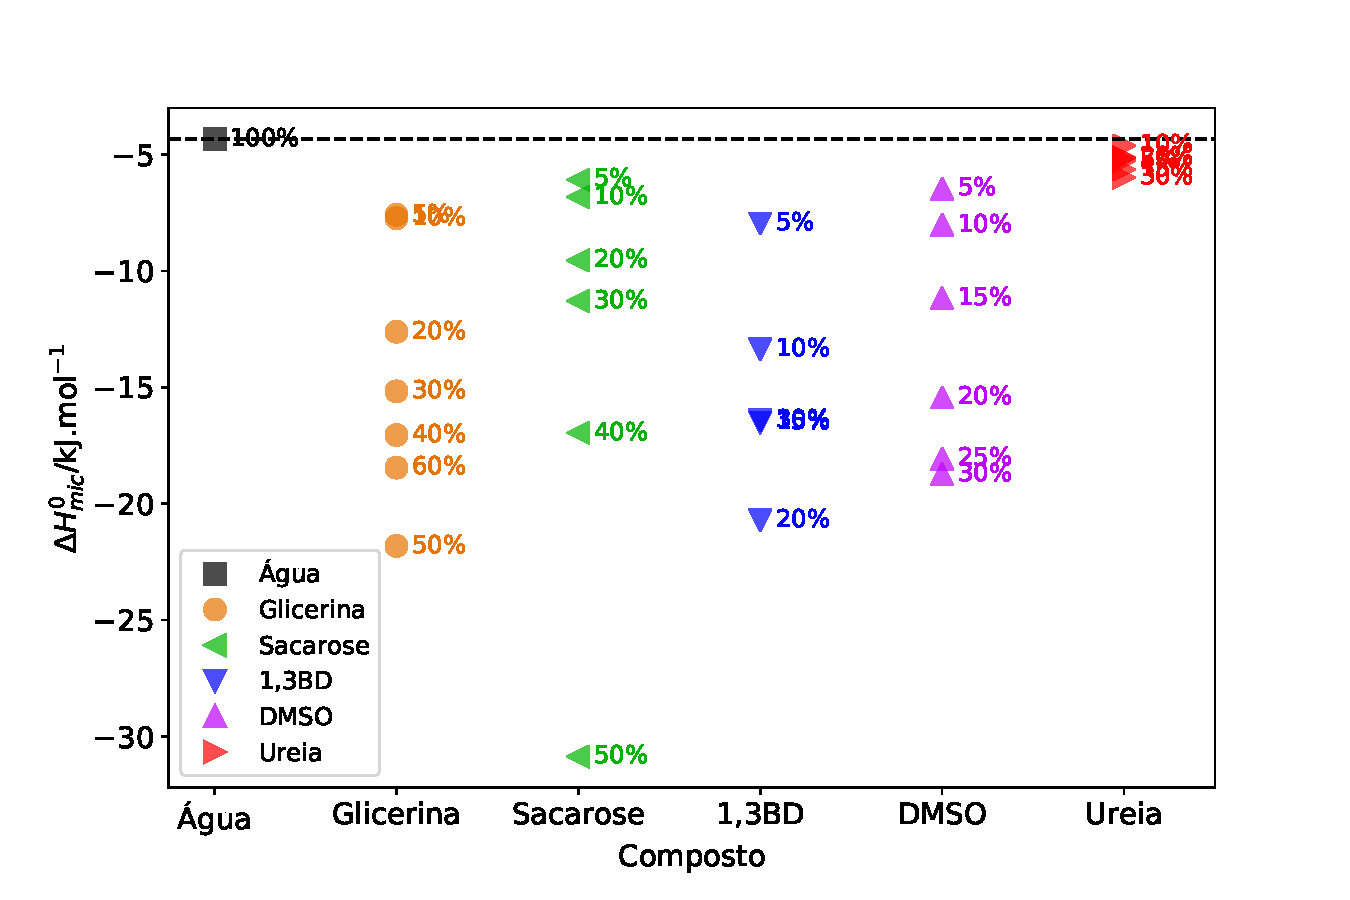
\includegraphics[width=\textwidth]{imagens/itc/DH_por_composto}
				\caption{\DHmic}
				\label{fig:dh_por_composto}
			\end{subfigure}
		
			\caption{\cmc{} e \DHmic{} para os vários aditivos}
			\label{fig:cmc_dh_por_composto}
		\end{figure}

		\begin{figure}[h]
			\begin{subfigure}[t]{0.5\textwidth}
				\centering
				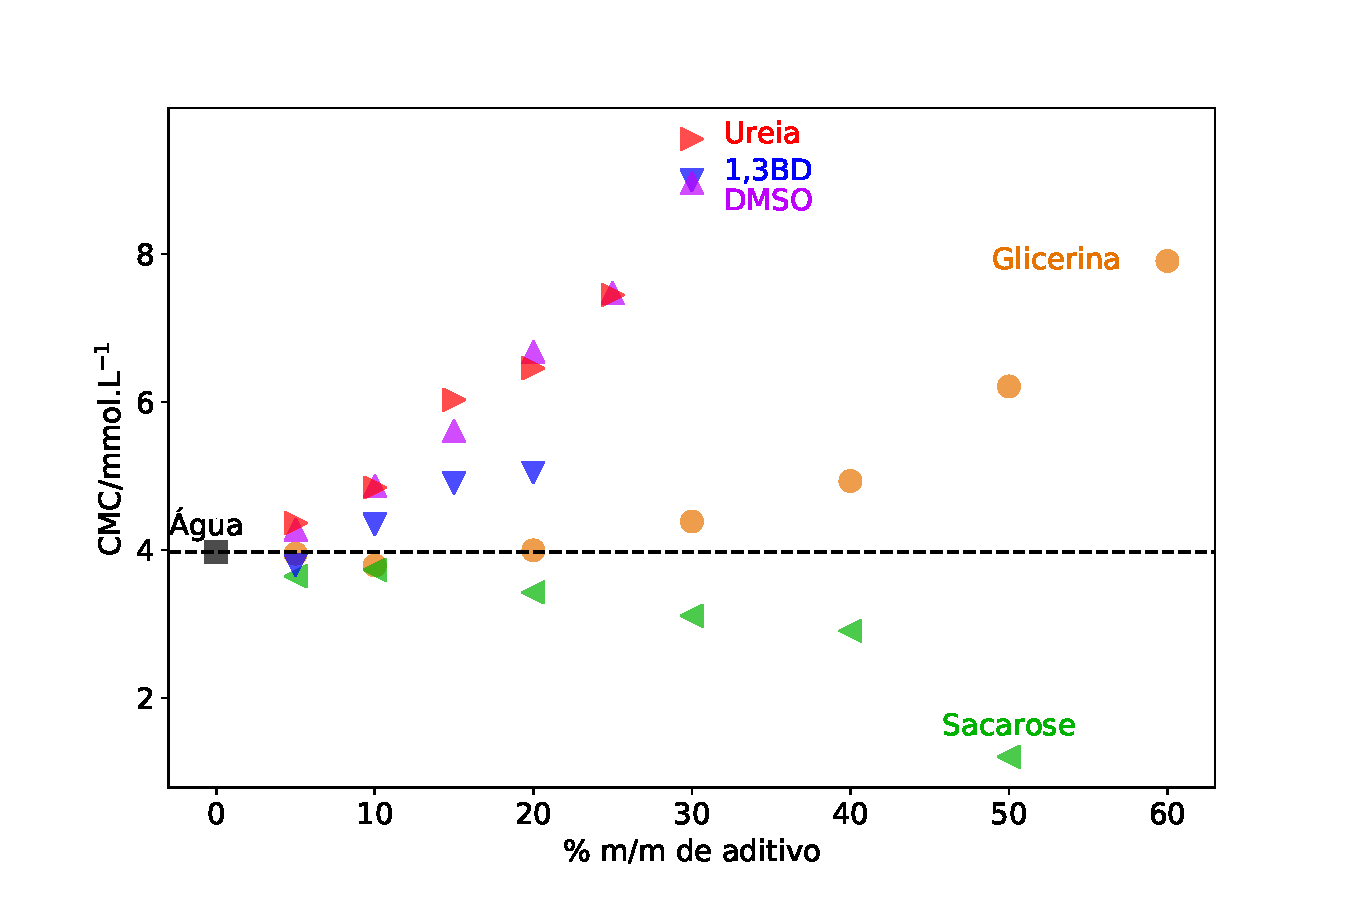
\includegraphics[width=\textwidth]{imagens/itc/ITC_cmc_adit}
				\caption{\cmc}
				\label{fig:cmc_por_conc}
			\end{subfigure} %
			\begin{subfigure}[t]{0.5\textwidth}
				\centering
				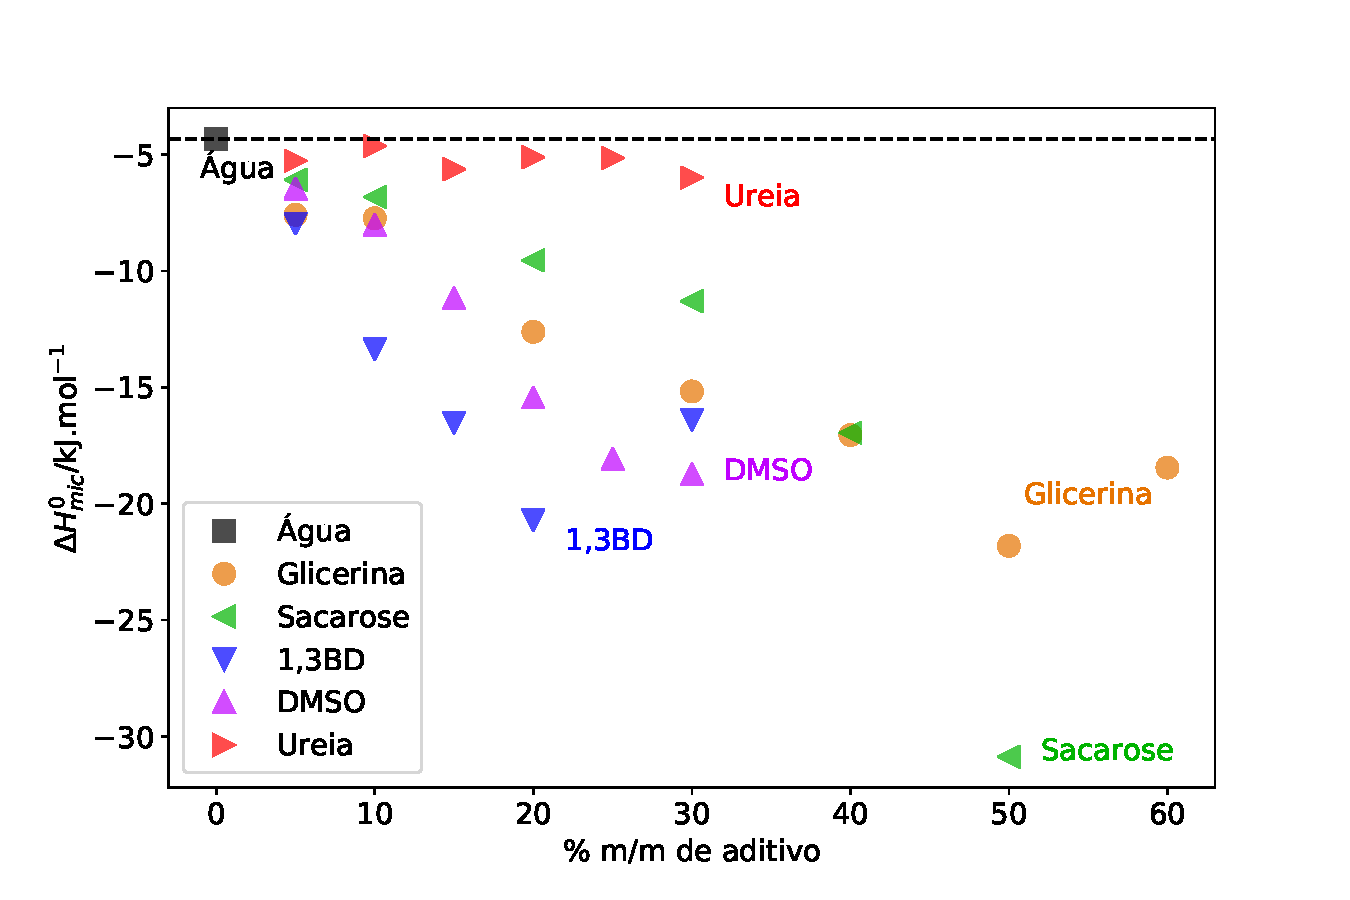
\includegraphics[width=\textwidth]{imagens/itc/ITC_DH_adit}
				\caption{\DHmic}
				\label{fig:dh_por_conc}
			\end{subfigure}
			
			\caption{\cmc{} e \DHmic{} em função da concentração de aditivo.}
			\label{fig:cmc_dh_por_conc}
		\end{figure}
	
		\FloatBarrier
		
	\chapter{Parâmetros a serem estudados}
		\section{Índice de refração}

		A figura \ref{fig:indice_refracao} mostrou como o índice de refração varia com a concentração de aditivo. Como os resultados reológicos evidenciaram, considerar somente o índice de refração não é uma maneira muito boa para explicar o comportamento reológico.
		
		Caso contrário, haveria um padrão notável num gráfico comparativo das concentrações e entalpias. Isso está evidenciado nas figuras \ref{fig:cmc_dh_por_n} e \ref{fig:cwlm_dhwlm_por_n}, onde não há um padrão geral observado para todos os aditivos.
		
		\begin{figure}[h]
			\begin{subfigure}[t]{0.5\textwidth}
				\centering
				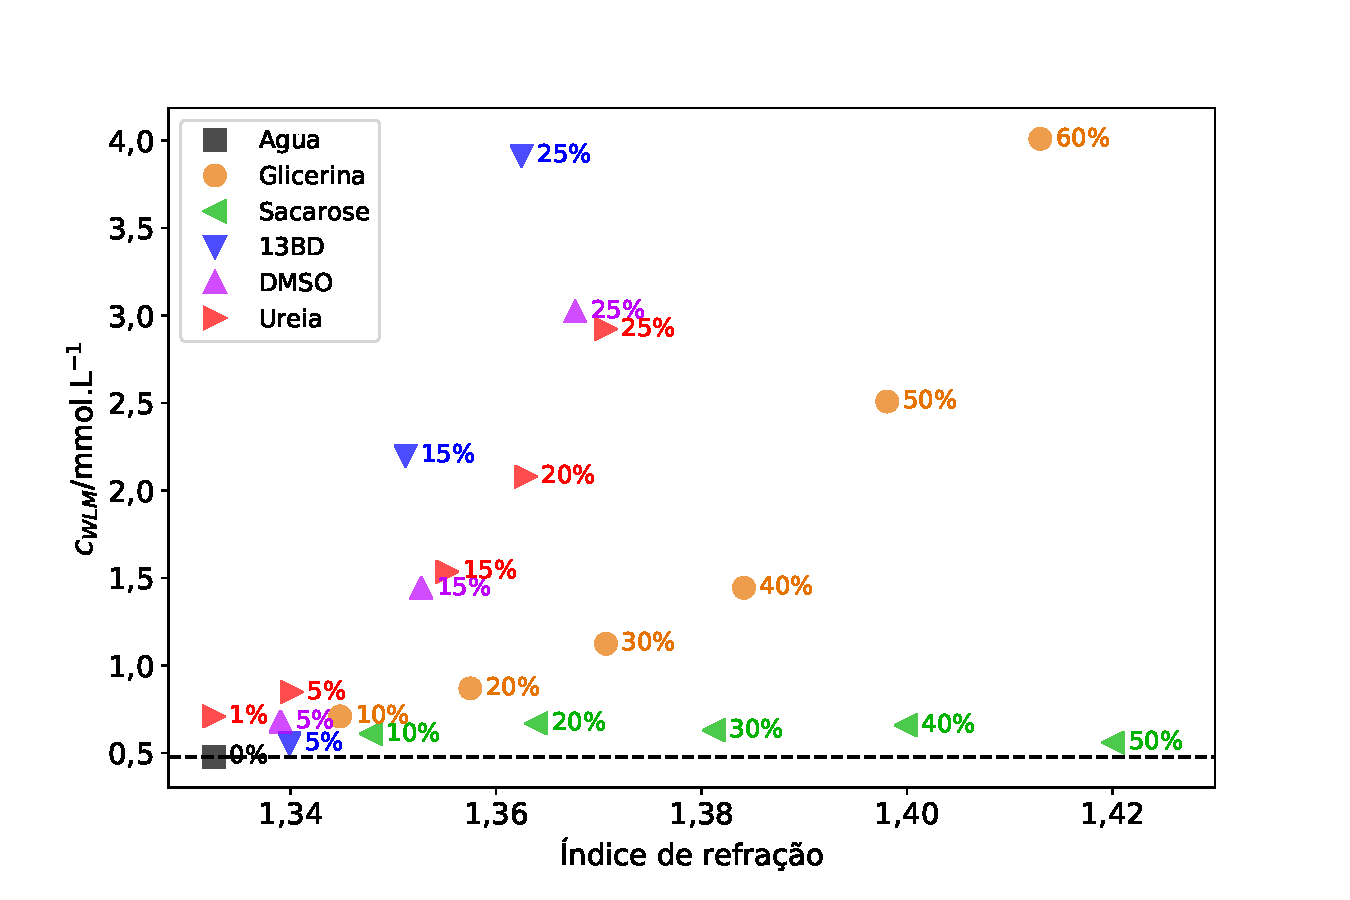
\includegraphics[width=\textwidth]{imagens/itc/Cwlm_por_n}
				\caption{\cwlm}
				\label{fig:cwlm_por_n}
			\end{subfigure} %
			\begin{subfigure}[t]{0.5\textwidth}
				\centering
				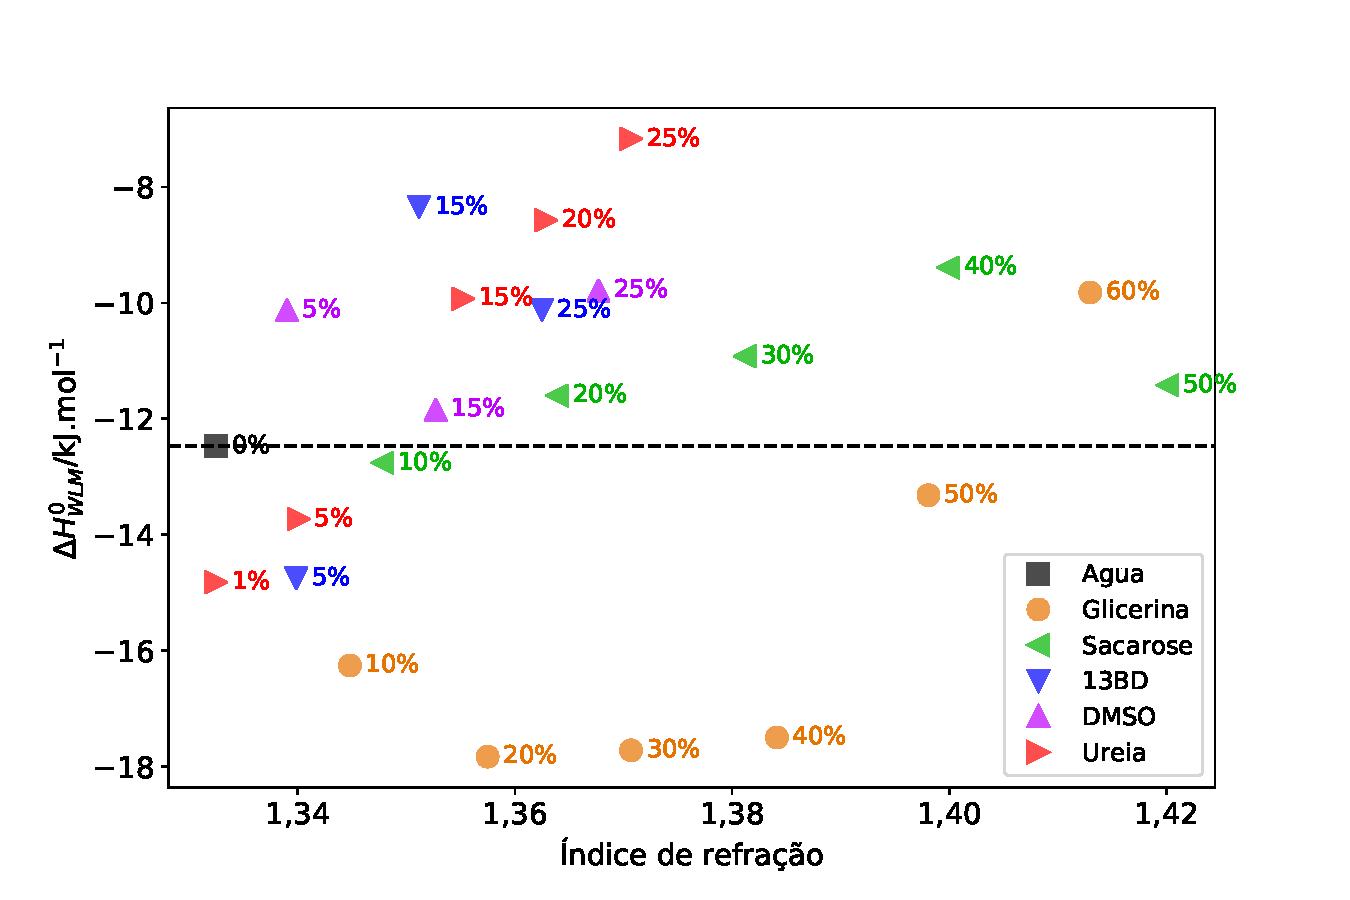
\includegraphics[width=\textwidth]{imagens/itc/DHwlm_por_n}
				\caption{\DHwlm}
				\label{fig:dhwlm_por_n}
			\end{subfigure}
			
			\caption{\cwlm{} e \DHwlm{} em função do índice de refração.}
			\label{fig:cwlm_dhwlm_por_n}
		\end{figure}
		
		\begin{figure}[h]
			\begin{subfigure}[t]{0.5\textwidth}
				\centering
				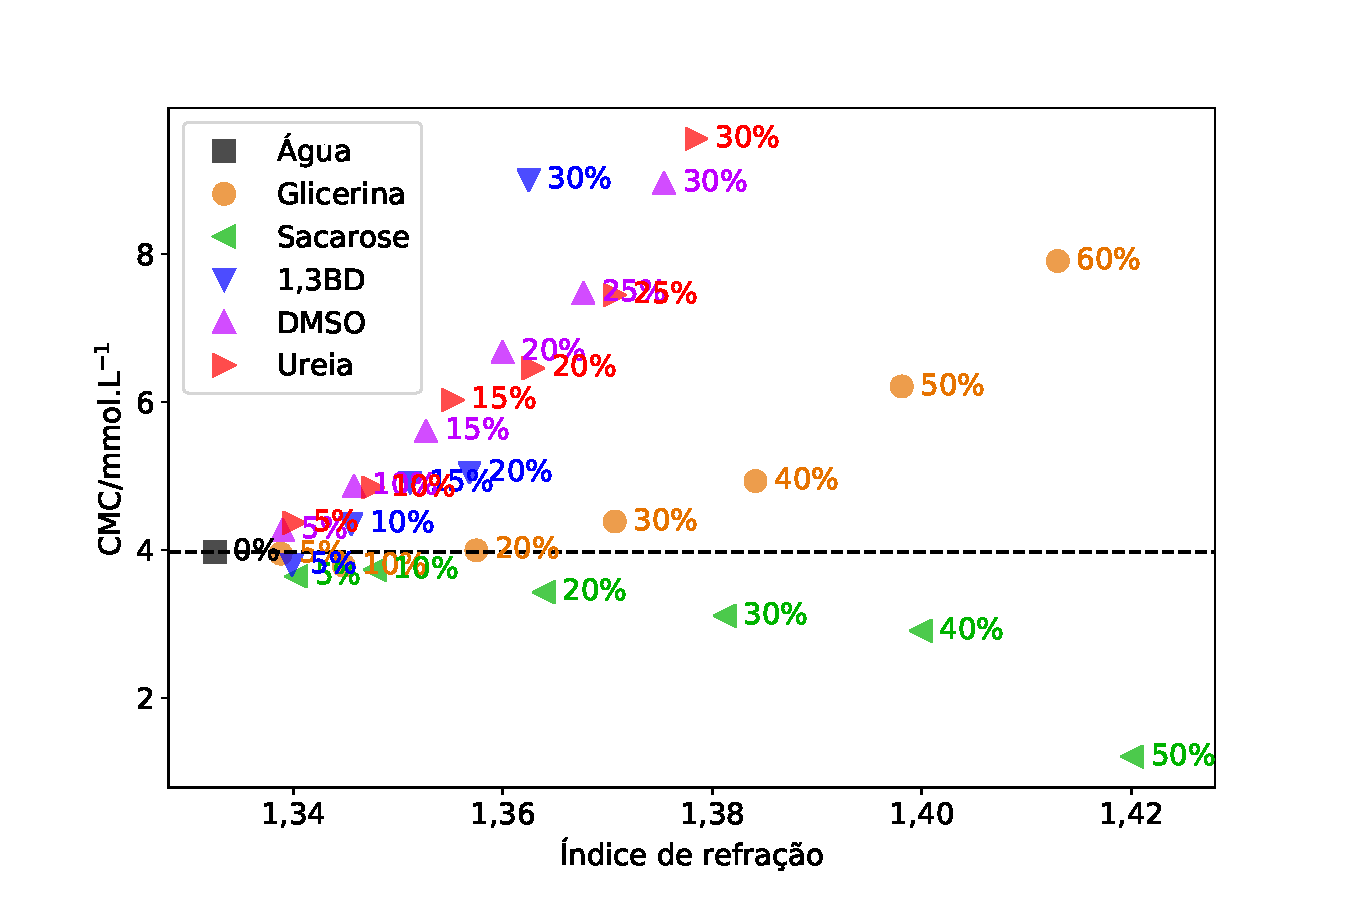
\includegraphics[width=\textwidth]{imagens/itc/CMC_por_n}
				\caption{\cmc}
				\label{fig:cmc_por_n}
			\end{subfigure} %
			\begin{subfigure}[t]{0.5\textwidth}
				\centering
				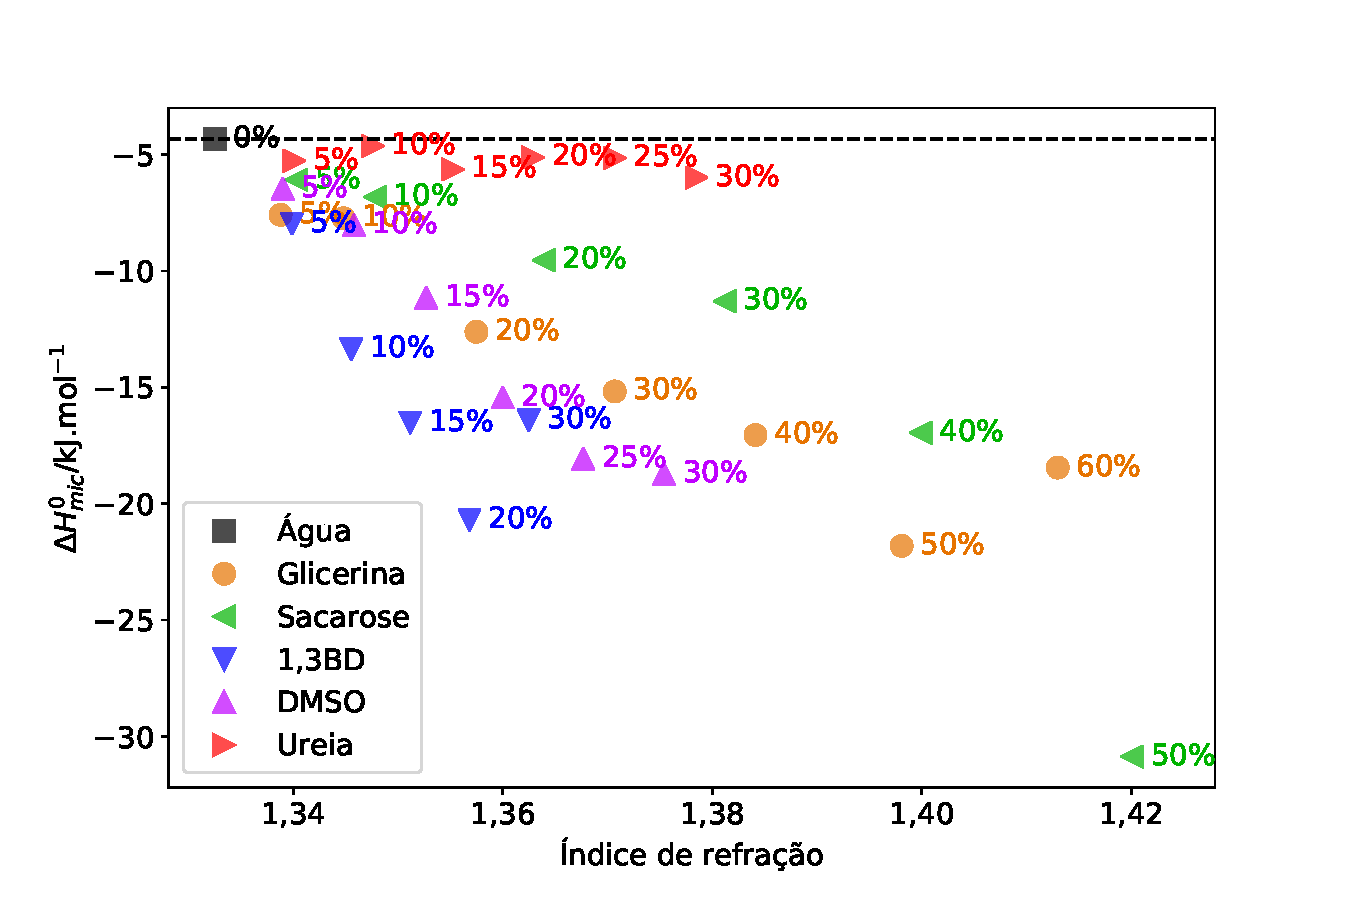
\includegraphics[width=\textwidth]{imagens/itc/DH_por_n}
				\caption{\DHmic}
				\label{fig:dh_por_n}
			\end{subfigure}
			
			\caption{\cmc{} e \DHmic{} em função do índice de refração.}
			\label{fig:cmc_dh_por_n}
		\end{figure}

		Comparando-se as figuras \ref{fig:cwlm_dhwlm_por_n} e \ref{fig:cmc_dh_por_n}, pode-se observar que há uma correlação entre a formação de micelas gigantes e as concentrações críticas. Aparentemente há um grupo composto de 1,3BD, DMSO e ureia. Glicerina e sacarose se comportam bastante diferentemente, sendo que sacarose possui o comportamento mais diferenciado, não havendo mudança na \cwlm{} e uma diminuição da \cmc{}.
		
		Agrupamentos desse tipo não podem ser feitos com as entalpias, que parecem ter valores bastante variáveis. Porém, é necessário enfatizar que os valores de entalpia obtidos para a formação de micelas gigantes não são tão confiáveis quanto os de formação de micelas esféricas. Para obter os perfis completos de formação de micelas gigantes, foi necessário aumentar a concentração de surfactante na seringa. Isso reduz a precisão na região inicial do perfil, onde é calculado o \DHwlm. Além disso, a resolução dos entalpogramas obtidos pelo calorímetro PEAQ é menor (39 pontos) do que no VP-ITC (90 pontos). Esse problema possui menor relevância para \cwlm{}, que foi definida como sendo o ponto mínimo da curva, não uma subtração de duas regiões pré e pós-micelar.  Apesar disso, o padrão observado para as mudanças de entalpia na presença de ureia podem ser explicadas pelo aumento da constante dielétrica do meio, como previamente mencionado.
	
		É interessante notar que as figuras que comparam as concentrações de formação e entalpias com o índice de refração (Figs. \ref{fig:cwlm_dhwlm_por_n} e \ref{fig:cwlm_dhwlm_por_conc}, \ref{fig:cmc_dh_por_n} e \ref{fig:cmc_dh_por_conc}) e a concentração de aditivo são bastante semelhantes. Isso se deve à dependência praticamente linear em baixas concentrações do índice de refração com a concentração de aditivo na escala mássica, um dos motivos para essa escalar ser escolhida.
		
		\FloatBarrier
		
		\section{Constante dielétrica}
		
		A constante dielétrica está relacionada ao grau de dissociação de espécies iônicas em solução. Quanto maior a constante, maior o grau de dissociação. Isso resulta, por exemplo, no aumento da \cmc{} pois há menos contraíons para reduzir a carga superficial micelar. A contribuição desse parâmetro já havia sido levantada em um estudo anterior. % todo: ref.
		A figura \ref{fig:cte_dieletrica} mostra como a constante dielétrica varia em função da concentração de aditivo. %todo: refs

		
		\begin{figure}[h]
			\centering
			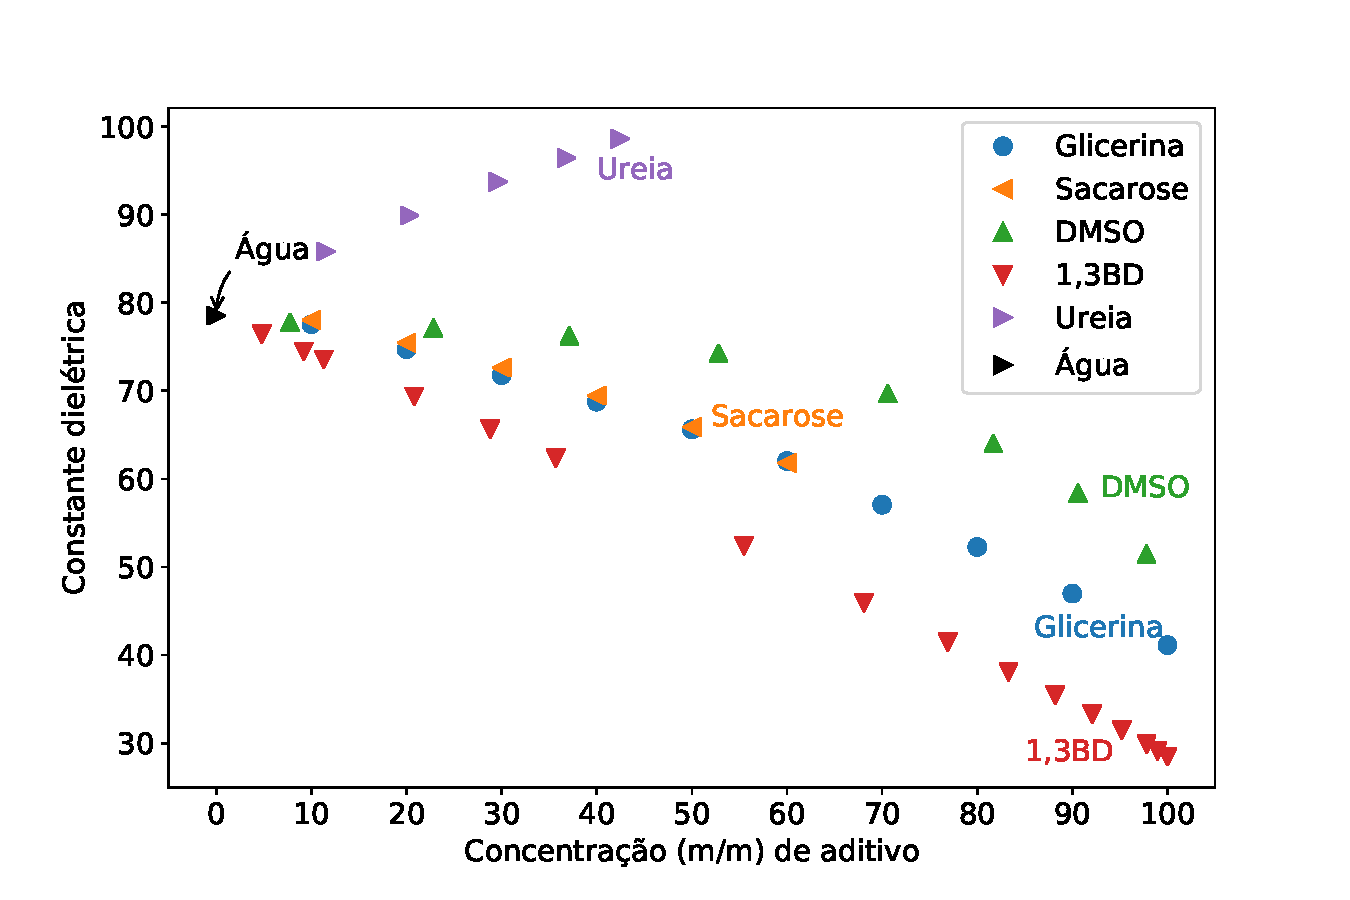
\includegraphics[width=0.7\textwidth]{imagens/propriedades/cte_dieletrica}
			\caption{Constante dielétrica em função da concentração de aditivo}  % todo: colocar quais são a 20°C e quais a 25°C
			\label{fig:cte_dieletrica}
		\end{figure}
	
		Não há variação entre o comportamento da sacarose e glicerina, e o DMSO praticamente não afeta a constante dielétrica na faixa de concentração estudada. O 1,3BD possui sempre os menores valores de \(\varepsilon\), o que indica que nessas soluções há a menor dessorção de contraíons da superfície micelar. O aditivo que afeta a constante dielétrica mais diferentemente dos outros é a ureia, que aumenta \(\varepsilon\). Isso se mostrará crucial para explicar seu comportamento diferenciado.
	
		Da mesma maneira que o índice de refração, os parâmetros dos ITCs serão comparados com a constante dielétrica do meio para tentar observar algum padrão.
		
		\begin{figure}[h]
			\begin{subfigure}[t]{0.5\textwidth}
				\centering
				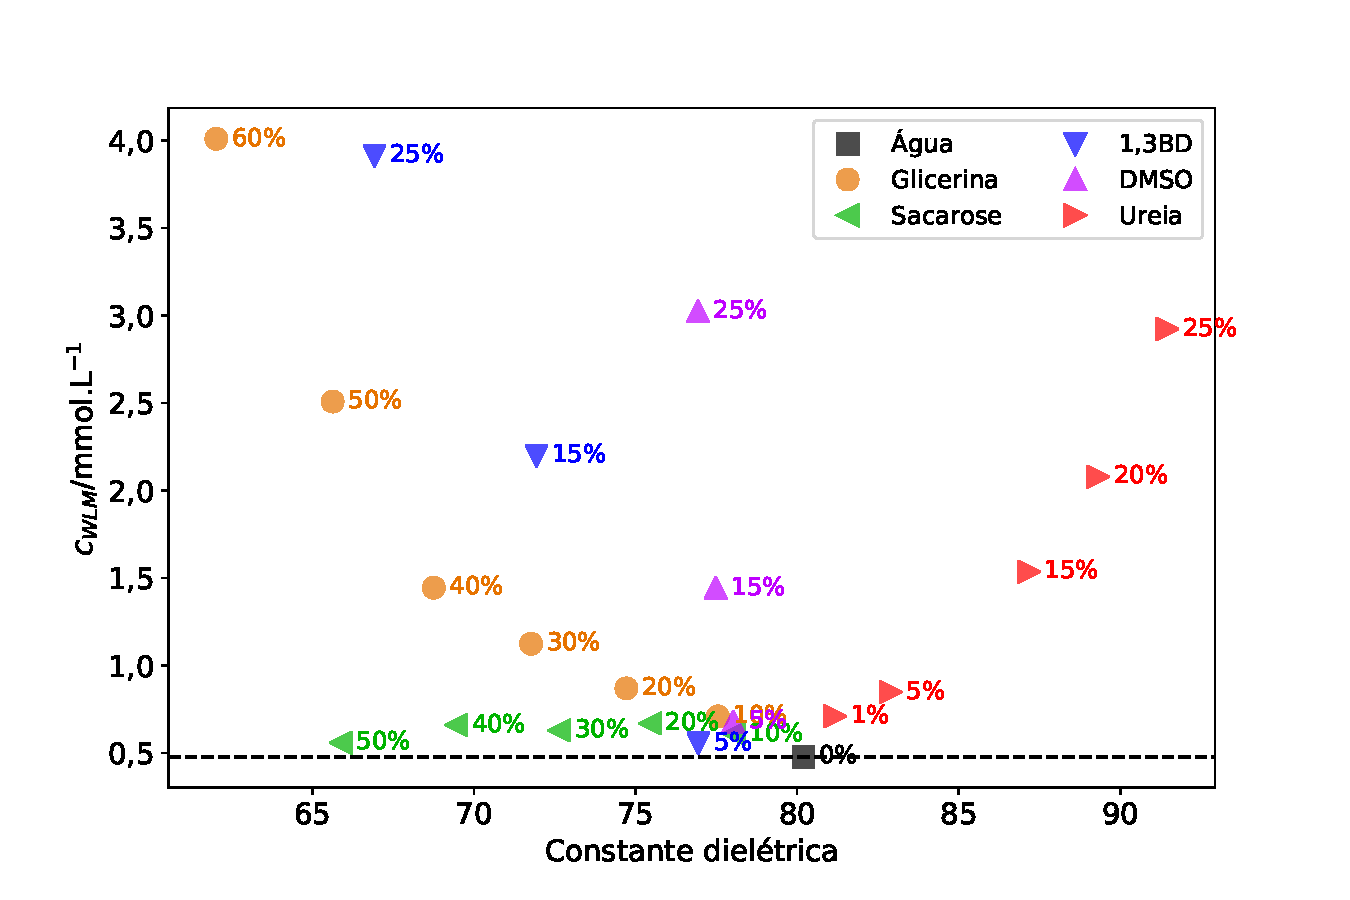
\includegraphics[width=\textwidth]{imagens/itc/Cwlm_por_eps}
				\caption{\cwlm}
				\label{fig:cwlm_por_eps}
			\end{subfigure} %
			\begin{subfigure}[t]{0.5\textwidth}
				\centering
				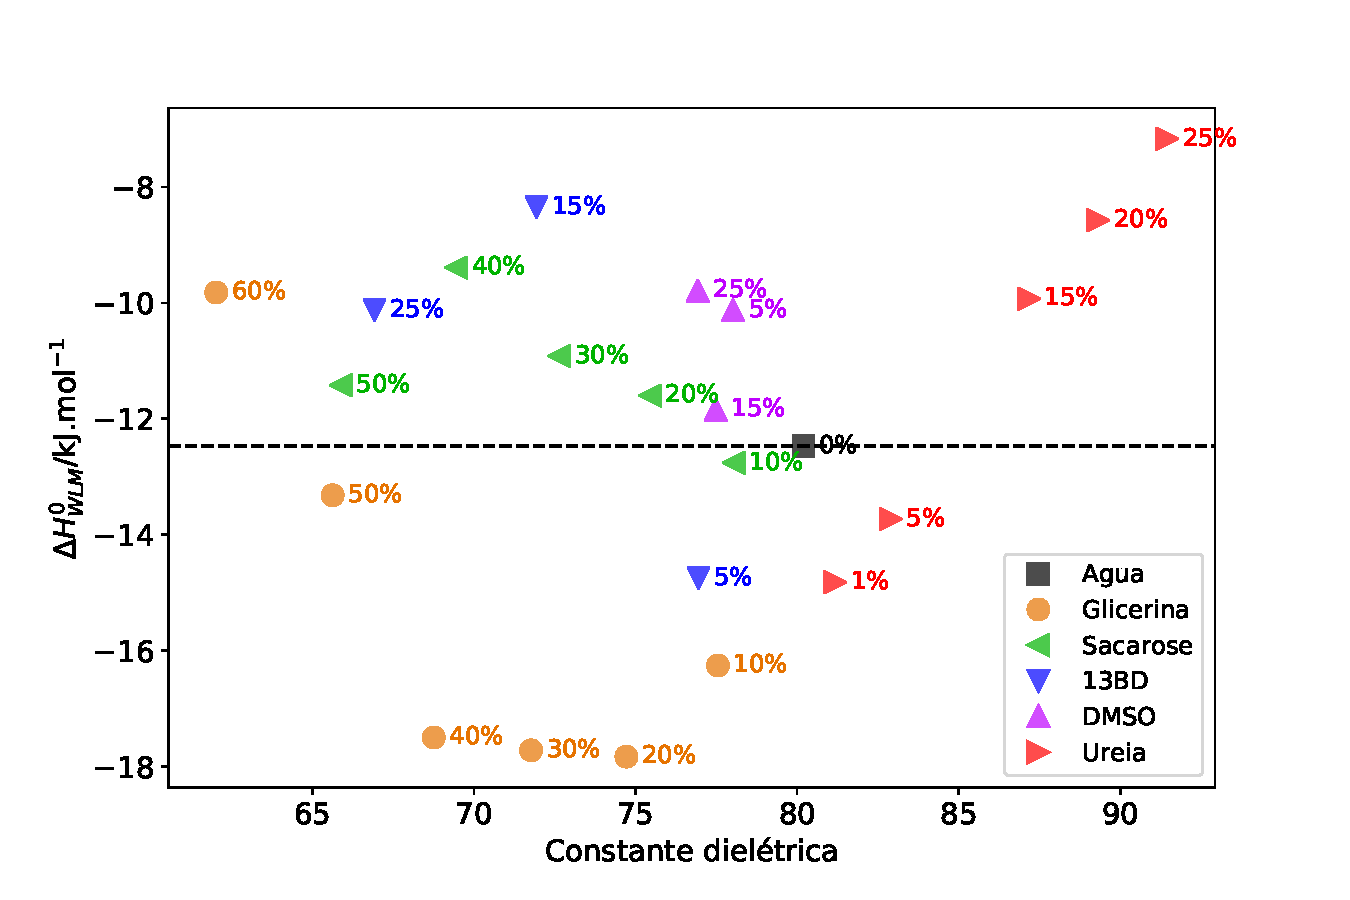
\includegraphics[width=\textwidth]{imagens/itc/DHwlm_por_eps}
				\caption{\DHwlm}
				\label{fig:dhwlm_por_eps}
			\end{subfigure}
			
			\caption{\cwlm{} e \DHwlm{} em função da constante dielétrica \(\varepsilon\).}
			\label{fig:cwlm_dhwlm_por_eps}
		\end{figure}
		
		\begin{figure}[h]
			\begin{subfigure}[t]{0.5\textwidth}
				\centering
				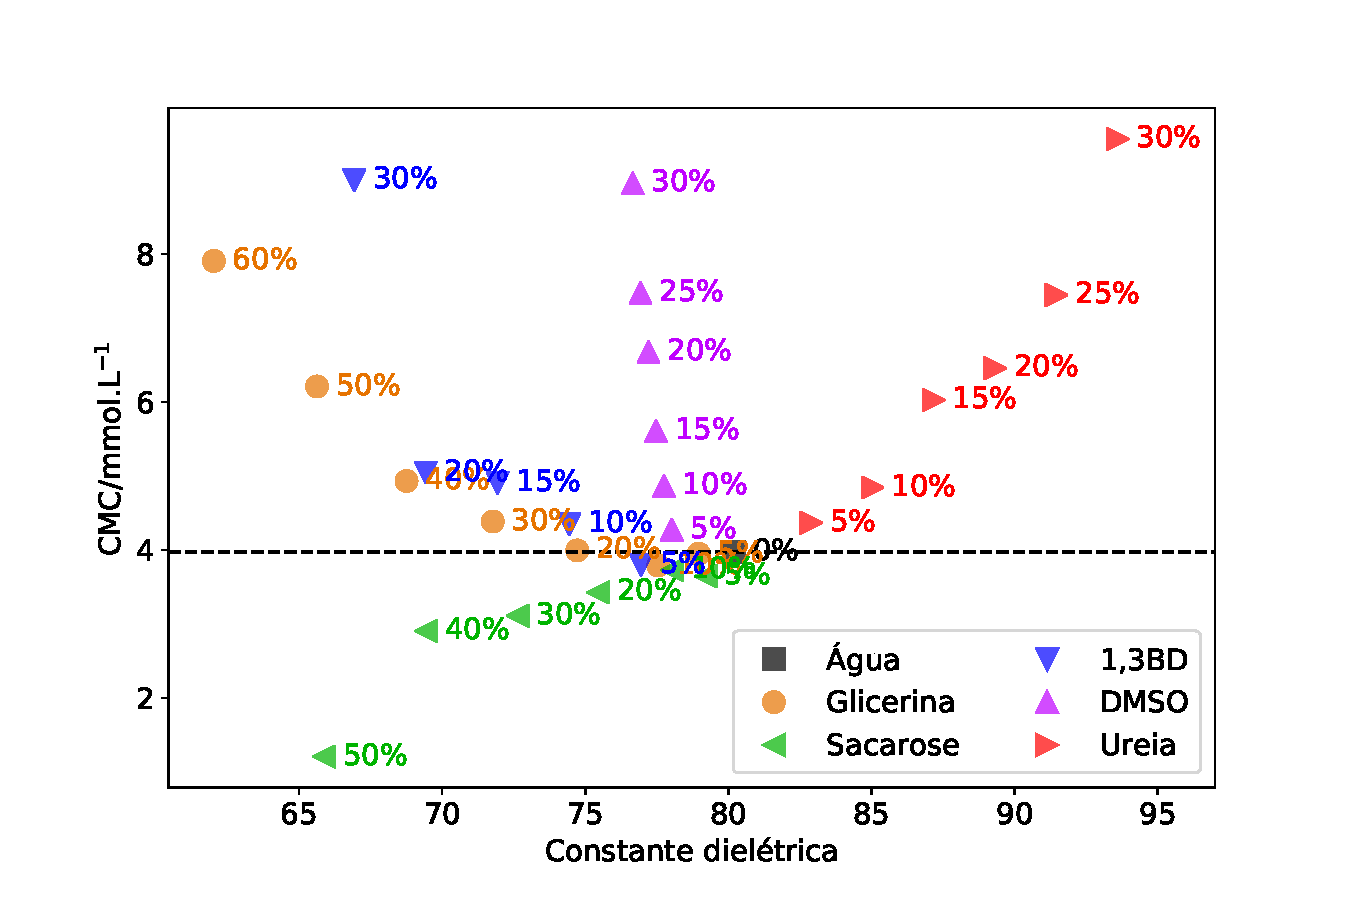
\includegraphics[width=\textwidth]{imagens/itc/CMC_por_eps}
				\caption{\cmc}
				\label{fig:cmc_por_eps}
			\end{subfigure} %
			\begin{subfigure}[t]{0.5\textwidth}
				\centering
				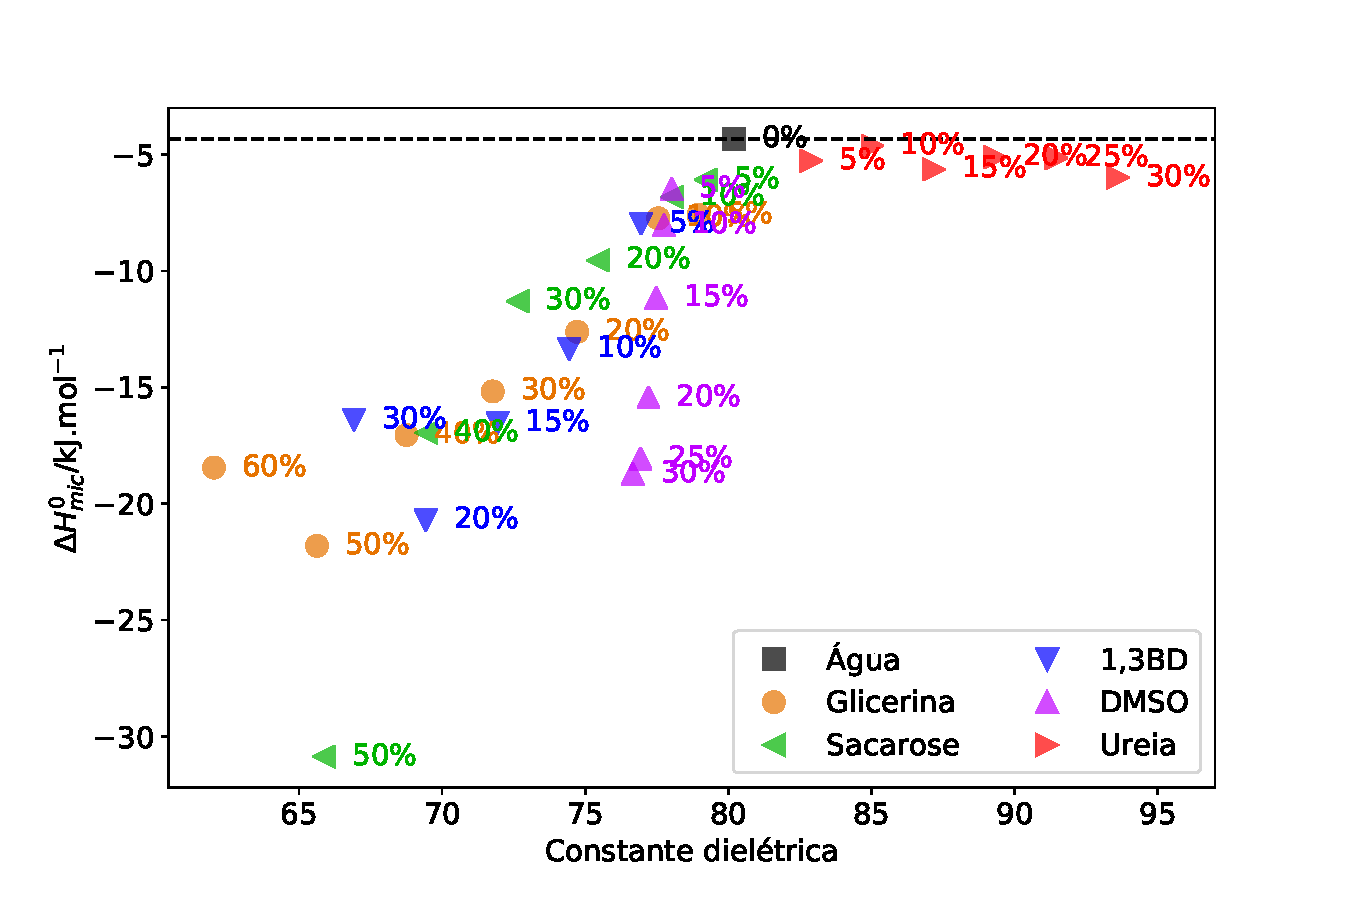
\includegraphics[width=\textwidth]{imagens/itc/DH_por_eps}
				\caption{\DHmic}
				\label{fig:dh_por_eps}
			\end{subfigure}
			\caption{\cmc{} e \DHmic{} em função da constante dielétrica \(\varepsilon\) do meio.}
			\label{fig:cmc_dh_por_eps}
		\end{figure}
		
		Algumas observações podem ser feitas quanto aos resultados observados. Aparentemente todos os aditivos possuem uma divergência única do ponto inicial, água, não havendo muita correlação entre eles, com exceção da \DHmic{}, onde a glicerina, sacarose e 1,3BD aparentam seguir uma tendência semelhante. A ureia, em todos os casos, diverge pois seu valor de constante dielétrica aumenta. O DMSO não afeta grandemente \(\varepsilon\), mas tanto as concentrações quanto entalpias são fortemente afetadas pelo aumento de sua concentração. Isso indica que a constante dielétrica, por si só, também não consegue explicar os fenômenos observados. Porém, ela é necessária para capturar a divergência observada com a ureia.
		
		% todo: mencionar reologia na seção do epsilon
		
		\FloatBarrier
		\section{Coesão do solvente e Parâmetro de Gordon}  % todo: falar sobre estruturação do solvente aqui
		
		Devido à incapacidade dos outros parâmetros explicarem o comportamento reológico e calorimétrico, procuramos por outras propriedades que possam estar relacionadas. Vendo trabalhos anteriores, pensamos na coesão do solvente para explicar o comportamento reológico e calorimétrico. Solventes bastante estruturados, como a água, diminuem a \cmc{} devido ao aumento da penalidade entrópica. Além disso, estipulamos que solventes melhor estruturados devem dificultar a locomoção das micelas gigantes durante os processos de reptação, aumentando a viscosidade aparente. A partir disso, foram coletadas informações sobre a coesão dos solventes utilizados.
		
		Glicerina na concentração de 43\% m/m possui uma probabilidade reduzida de ligações de hidrogênio, portanto a percolação da rede de ligações de hidrogênio é reduzida. Já açúcares são desestruturadores em baixas concentrações e estruturadores em altas. Para a glicose, a estruturação acontece em torno de 25-30\% m/m, já outros estudos mencionam 37\% m/m. Sacarose foi descrita em trabalhos anteriores como aditivo para aumento da separação interlamelar, semelhante à glicerina. É possível que a sacarose afete as micelas e não as bicamadas devido à maior área de contato das micelas com o solvente. Além disso, a reologia observa a dinâmica das micelas ao fluir pelo solvente, já a distância interlamelar é uma propriedade estática, e seria melhor comparada com uma distância intermicelar média.
		
		DMSO foi demonstrado como um agente desestruturador em altas concentrações e estruturador em baixas, e essas propriedades foram descritas como fracas frente à capacidade do DMSO em solubilizar moléculas de surfactante. % todo: o que significa isso exatamente?
		Já o papel da ureia é inconclusivo de acordo com a literatura, com vários mecanismos propostos em estudos. % todo: mencionar os três mecanismos.
		
		Para seguir a lógica das discussões na outra seção, é necessário levantar uma propriedade que traduza o conceito de coesão do solvente para um número mensurável. O parâmetro de Gordon já foi utilizado na literatura com esse propósito, então ele será utilizado neste trabalho. Porém, é necessário reforçar que esse parâmetro não traduz perfeitamente o conceito de estruturação, e será utilizado mais como uma maneira para facilitar a discussão. O parâmetro de Gordon é definido pela Eq. \ref{eqn:Gordon}, onde \(\gamma\) é a tensão superficial do líquido e \(\bar{V}_m\) é o volume molar médio do líquido, definido pela Eq. \ref{eqn:volume_molar_médio}. 
		
		\begin{equation}
			G = \dfrac{\gamma}{\bar{V}_m^{\frac{1}{3}}}
			\label{eqn:Gordon}
		\end{equation}
		
		\begin{equation}
			\bar{V}_m = \bar{V}_{m_{1}}x_1 + \bar{V}_{m_{2}}x_2
			\label{eqn:volume_molar_médio}
		\end{equation}
		
		Amostras com as composições desejadas foram preparadas e suas tensões superficiais foram medidas em quintuplicatas. As tensões obtidas estão na figura \ref{fig:tensao_superficial_por_conc} e os valores do parâmetro de Gordon obtidos estão na figura \ref{fig:param_gordon_por_conc}.
		
		\begin{figure}[h]
			\centering
			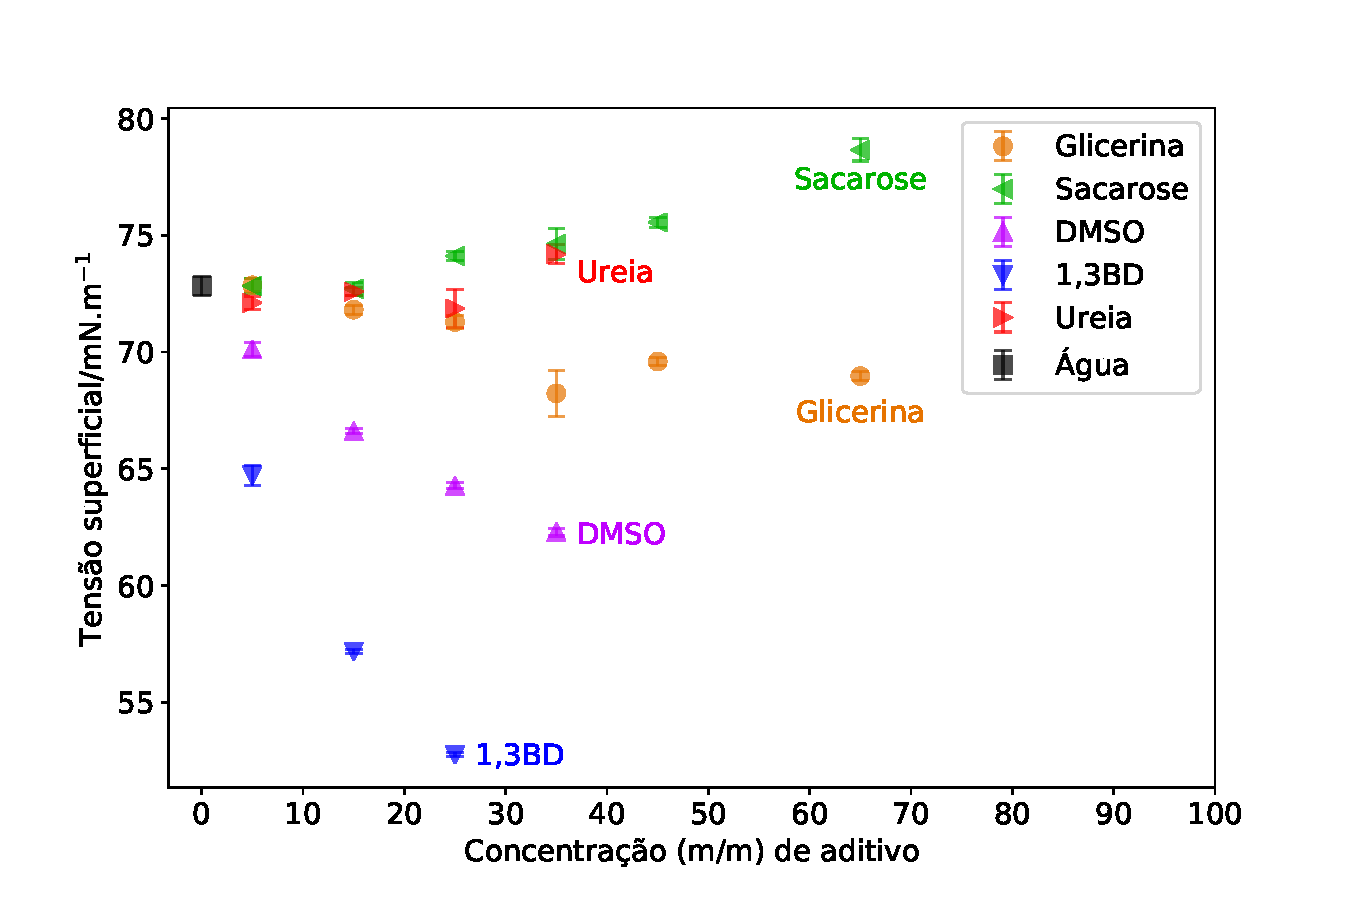
\includegraphics[width=0.7\textwidth]{imagens/propriedades/tensao_superficial}
			\caption{Tensão superficial de misturas binárias dos aditivos em água}
			\label{fig:tensao_superficial_por_conc}
		\end{figure}
		
		\begin{figure}[h]
			\centering
			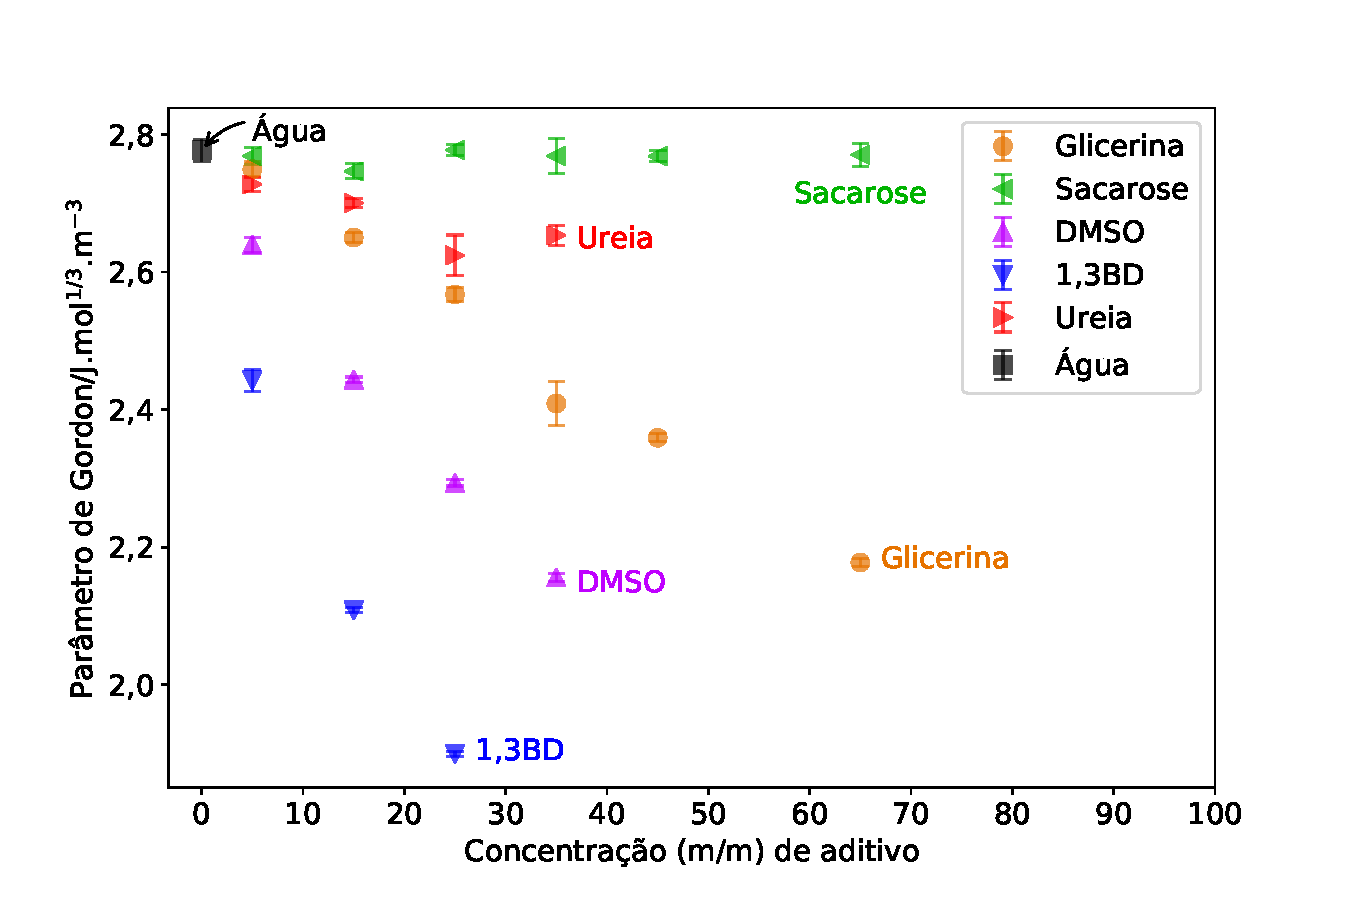
\includegraphics[width=0.7\textwidth]{imagens/propriedades/param_gordon}
			\caption{Parâmetro de Gordon das misturas binárias dos aditivos em água}
			\label{fig:param_gordon_por_conc}
		\end{figure}
		
		Podemos observar que os dois gráficos possuem basicamente o mesmo formato. A maior alteração ocorre devido à divisão pelo volume molar, onde a alta massa da sacarose mascara o aumento de sua tensão superficial, tornando os valores de \(G\) constantes. Essa divisão também diferencia as curvas de ureia e sacarose.
		
		Pelo posição relativa das retas observadas para cada aditivo, podemos construir a seguinte correlação de estruturação do solvente:
		
		\begin{equation*}
			\textrm{1,3BD} < \textrm{DMSO} < \textrm{Glicerina} < \textrm{Ureia} < \textrm{Sacarose}
		\end{equation*}
		
		Essa sequência possui grande correlação com o comportamento reológico (com exceção da ureia). 1,3BD, que possui a menor estruturação, reduz mais fortemente a viscosidade das micelas. Já a sacarose praticamente não afetou a estruturação do solvente, e também não afetou muito a viscosidade. Como mencionado, a ureia é uma exceção devido à grande alteração na constante dielétrica, que deve dessorver moléculas de salicilato das micelas e aumentar sua carga. Isso faz com que o mecanismo principal de relaxação seja a reptação na faixa de concentração estudada, então a viscosidade é sempre alta.
		
		Para compreender o efeito do parâmetro de Gordon nas titulações, foram criadas figuras comparativas, da mesma maneira que nas seções anteriores. Os comparativos para a formação de micelas gigantes e micelas esféricas estão nas figuras \ref{fig:cwlm_dhwlm_por_g} e \ref{fig:cmc_dh_por_g}, respectivamente.
		
		\begin{figure}[h]
			\begin{subfigure}[t]{0.5\textwidth}
				\centering
				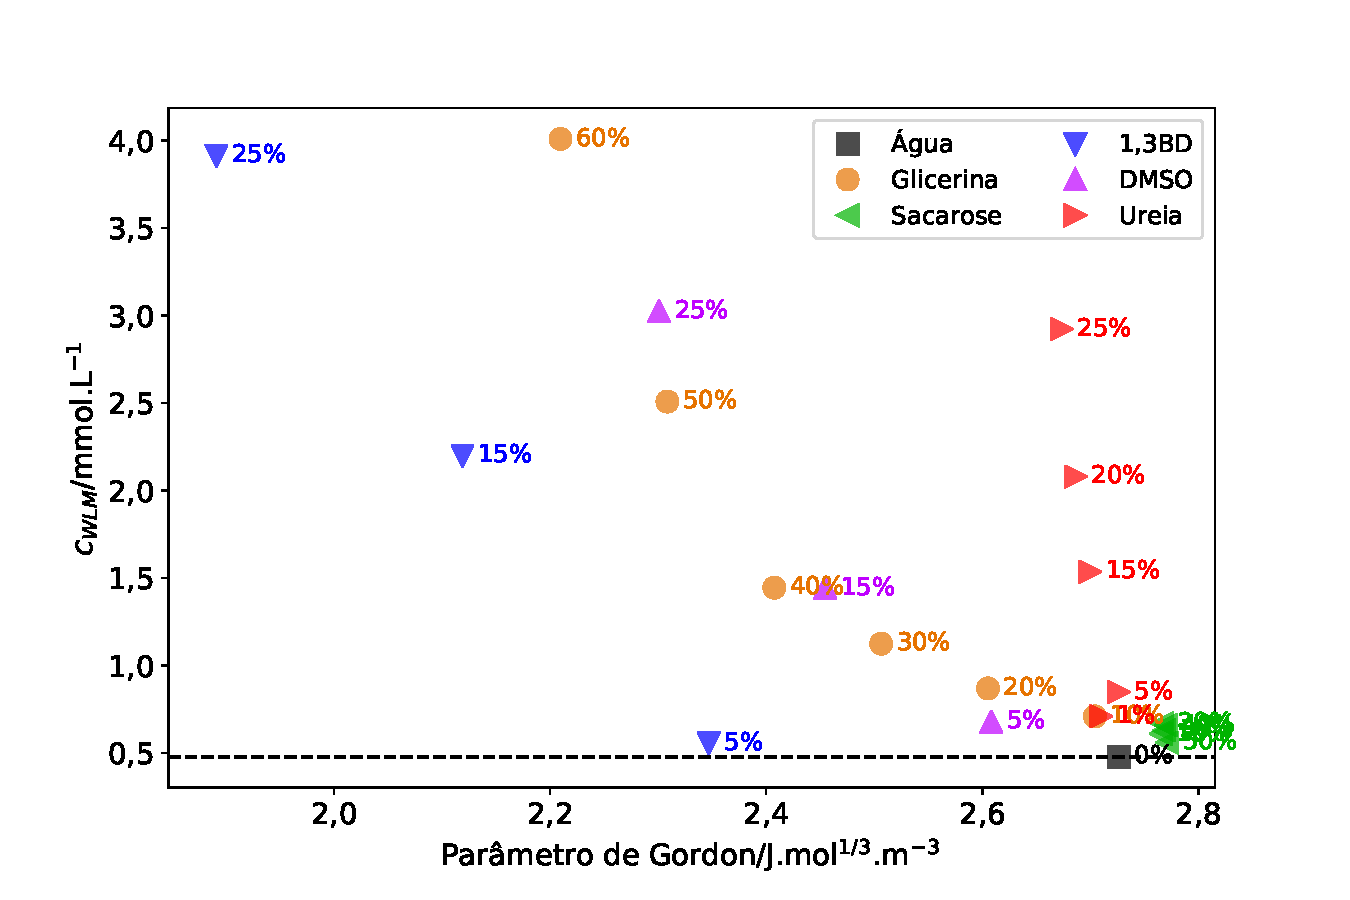
\includegraphics[width=\linewidth]{imagens/itc/Cwlm_por_G}
				\caption{\cwlm}
				\label{fig:cwlm_por_g}
			\end{subfigure} %
			\begin{subfigure}[t]{0.5\textwidth}
				\centering
				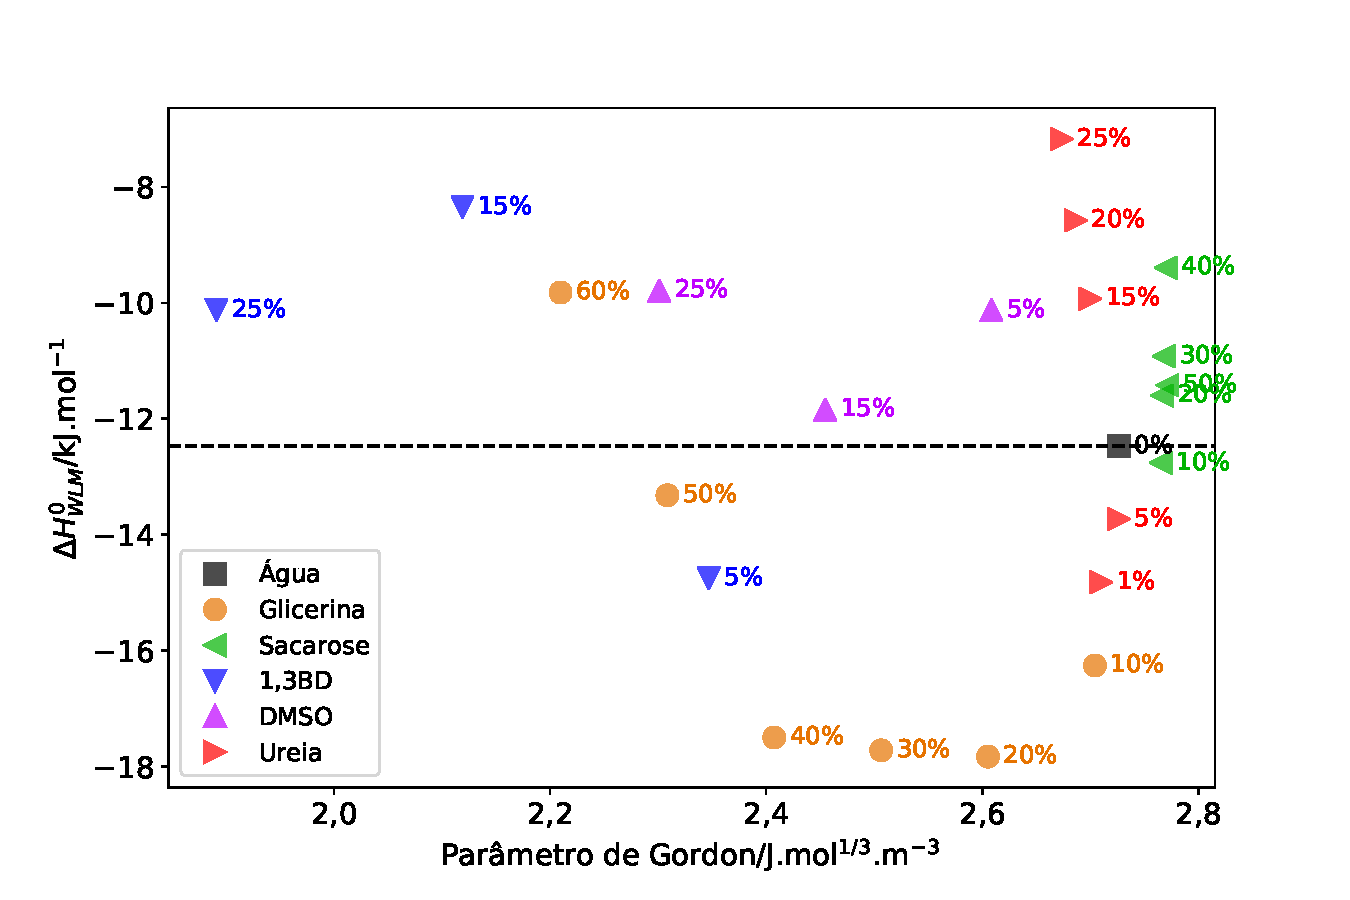
\includegraphics[width=\textwidth]{imagens/itc/DHwlm_por_G}
				\caption{\DHwlm}
				\label{fig:dhwlm_por_g}
			\end{subfigure}
			\caption{\cwlm{} e \DHwlm{} em função do parâmetro de Gordon}
			\label{fig:cwlm_dhwlm_por_g}
		\end{figure}
		
		\begin{figure}[h]
			\begin{subfigure}[t]{0.5\textwidth}
				\centering
				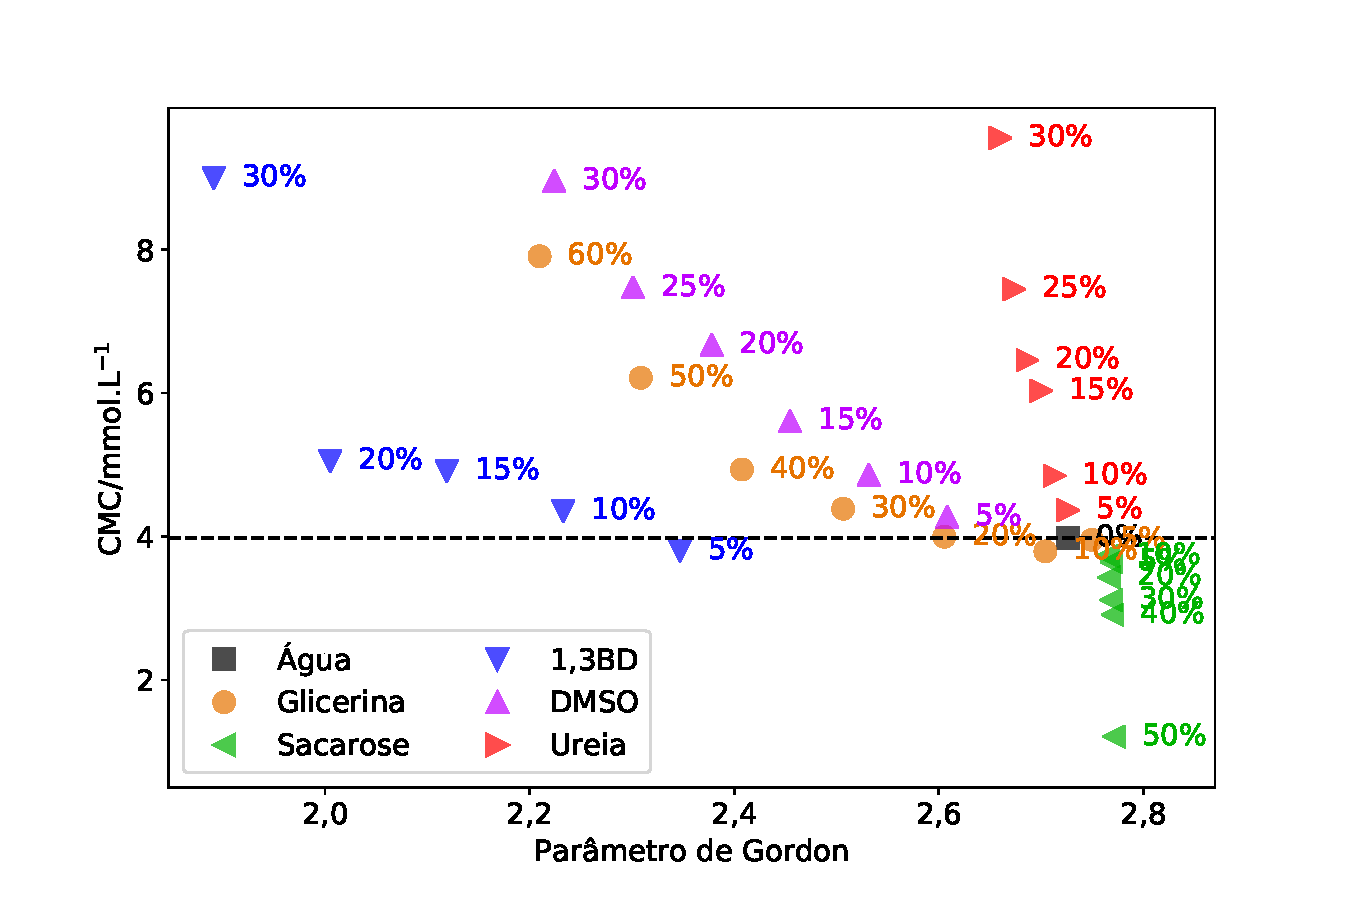
\includegraphics[width=\textwidth]{imagens/itc/CMC_por_G}
				\caption{\cmc}
				\label{fig:cmc_por_g}
			\end{subfigure} %
			\begin{subfigure}[t]{0.5\textwidth}
				\centering
				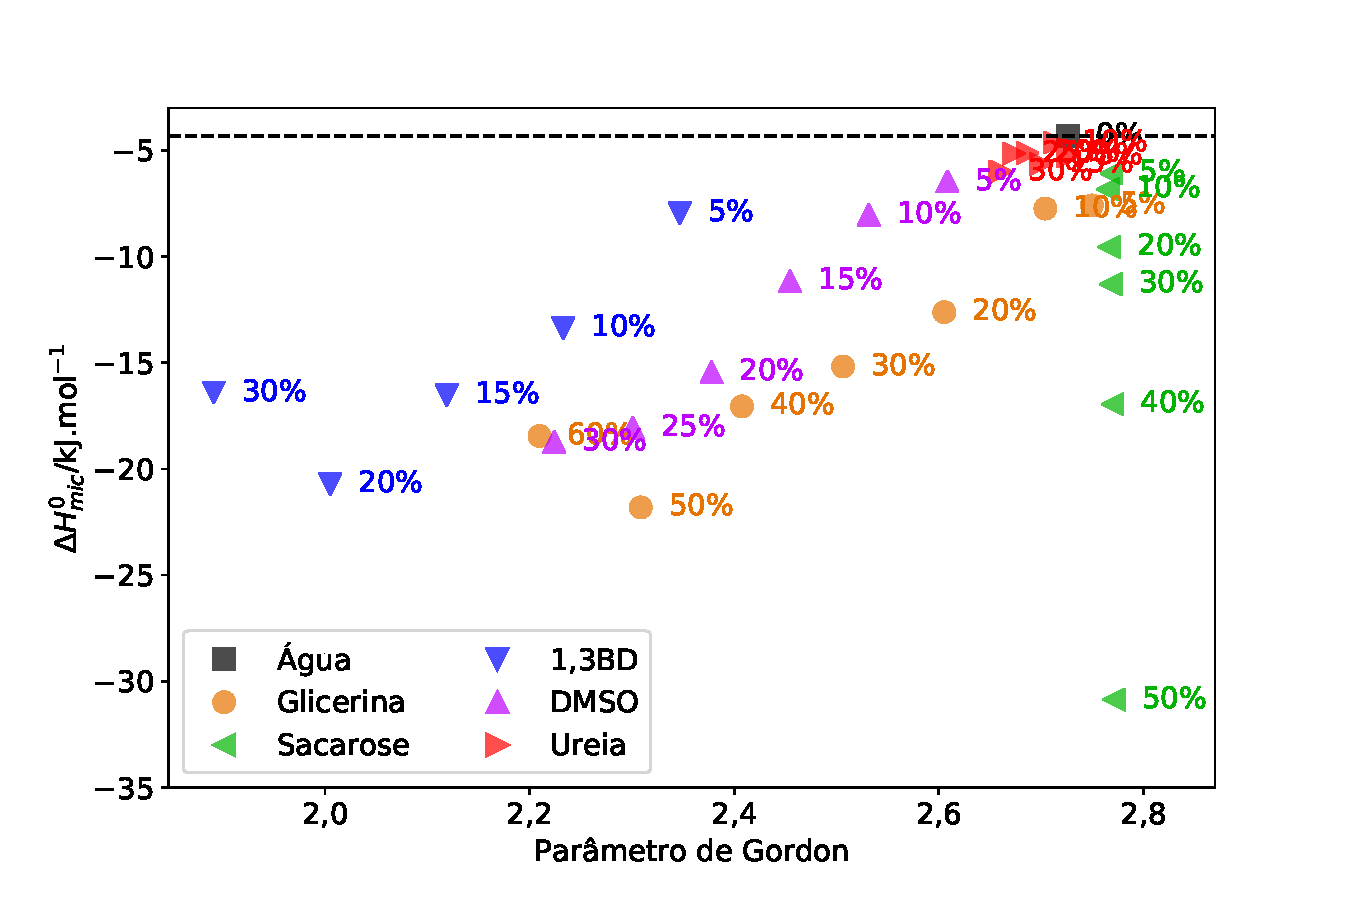
\includegraphics[width=\linewidth]{imagens/itc/DH_por_G}
				\caption{\DHmic}
				\label{fig:dh_por_g}
			\end{subfigure}
			\caption{\cmc{} e \DHmic{} em função do parâmetro de Gordon}
			\label{fig:cmc_dh_por_g}
		\end{figure}
		
		Pela inclinação das retas observadas nas figuras \ref{fig:cwlm_por_g} e \ref{fig:cmc_por_g}, podemos observar o quão forte é o efeito de uma mudança no parâmetro de Gordon do aditivo específico na concentração de micelização. A ureia possui o efeito mais forte, onde uma pequena variação de \(G\) aumentou muito a \cmc, porém isso se deve principalmente ao aumento de \(\varepsilon\). Sacarose não afetou a \cwlm{} e diminuiu a \cmc, pelas razões já discutidas. Os outros três aditivos seguem uma tendência semelhante, onde uma diminuição de \(G\) resulta no aumento gradativo de \cwlm{} e \cmc. Pela inclinação, 1,3BD possui o efeito mais brando na \cwlm, mas se a concentração de aditivo for levada em consideração também, vemos que seu efeito é bastante forte, atingindo a \cwlm{} de 4 \mM{} com 25\% de aditivo, comparado com glicerina, que atingiu essa concentração com 60\%. Interessantemente, até 20\%, o efeito do 1,3BD na \cmc{} é bastante pequeno, menor que o DMSO, e há um salto em 30\%, equiparando-se ao DMSO.
				
		As \DHwlm{} não possuem uma ordenação clara. Ureia aparenta ter comportamentos divergentes entre soluções de concentrações baixas (\(<\) 15\%) e altas (\(\ge\) 15\%). Já a \DHmic{} possui padrões, como os valores de ureia agrupados, pois não há salicilato para ser dessorvido. Glicerina e DMSO novamente possuem um comportamento relativemente próximo, e 1,3BD tem o menor efeito na entalpia por variação de \(G\). A sacarose diminui a \DHmic{} e a \cmc{}, apesar de não afetar \(G\), indicando que seu papel está relacionado com a interação com as micelas, não somente seu efeito no solvente.
		
		A correlação do parâmetro de Gordon é especialmente forte com o comportamento reológico, e há algumas correlações que podem ser feitas com a calorimetria. Deve ser enfatizado que esse parâmetro, por si só, também não explica o comportamento completo. É necessário combinar todas essas considerações para entender o sistema.
		\FloatBarrier
		
		\section{Interação dos aditivos com a superfície micelar}
		% todo: pensar em desmembrar essas considerações e espalhar nas outras seções
		
		Uma propriedade importante que deve receber enfoque é a interação dos aditivos com a superfície micelar. Aditivos que interagem fortemente afetam muito os processos de autoassociação, como demonstra o salicilato de sódio. Efeitos semelhantes, mas menos intensos, podem complementar os parâmetros levantados até o momento.
		
		Estudos da influência de álcoois lineares na viscosidade de micelas gigantes de C\textsubscript{16}TASal e CPySal mostraram que quando álcoois de cadeia curta interagiam com a superfície micelar, agiam como um cossolvente e diminuiam o comprimento das micelas, logo diminuindo sua viscosidade. Caso 1,3-BD se comporte de maneira similar, esse é mais um efeito que pode resultar nas quedas fortes da viscosidade. Um estudo mostra que o 1,3-BD interage como cosurfactante em cristais líquidos, o que reforça a teoria de seu efeito em micelas gigantes. Além disso, o 1,3BD pode interagir com os grupos metil na superfície micelar, diminuindo a atração entre as micelas que ocorre devido a esses grupos, o que diminuiria a viscosidade. A glicerina, por ser mais polar, possivelmente não tem o mesmo efeito que 1,3BD, logo é menos eficaz em diminuir a viscosidade ou aumentar a \cmc. O DMSO pode se solubilizar na superfície micelar e interagir com os grupos metila, pois é menos polar que os outros aditivos, e isso pode resultar em uma diminuição maior na viscosidade. 
		
		%Ureia interage fortemente com a superfície micelar, mas não como agente intercalante. % todo: verificar o artigo na ACS Omega sobre o que eu falo sobre isso.
	%	A concentração de ureia na superfície é cerca de 10-30\% menor do que no seio da solução. 
		
		% todo: refs
		A sacarose diminui a \cmc{} de outros surfactantes, como SDS, CTAB e Brij 35, pela interação de suas hidroxilas com a superfície micelar reduzindo a repulsão, e pela estruturação do solvente. Logo, a diminuição de \(n\) e \(\varepsilon\), que deveriam aumentar a \cwlm{}, são compensadas e a \cwlm{} é mantida. Não há uma diminuição de \cwlm, como houve de \cmc, pois o salicilato interage mais fortemente com a superfície micelar, deslocando as hidroxilas da sacarose, logo seu efeito é principalmente na estruturação do solvente.

		\section{Correlações simultâneas dos parâmetros com \cmc{} e \DHmic}
		% todo: colocar que os gráficos resultantes são 4D
		
		Até este momento, foram feitas correlações dos parâmetros do solvente com as propriedades calorimétricas mensuradas somente um a um, com raros casos explicados considerando-se outros parâmetros. Seria interessante tentar correlacionar todas essas propriedades simultaneamente, ou seja, realizar uma análise multivariada.
		
		\subsection{PLS}
		
		Foram feitas análises de PLS (\emph{Partial Least Squares}) com o índice de refração, constante dielétrica e parâmetro de Gordon para tentar prever a \cmc{} e a \DHmic. Utilizou-se dois componentes principais (de 3) em ambos os casos, os dados foram autoescalados de modo a garantir que todas as parâmetros tenham o mesmo peso no modelo final. Utilizou-se validação cruzada com 1 elemento, e sem validação cruzada, e o vetor de previsão permaneceu igual. Essas análises foram realizadas com o software Pirouette 3.11, e comparadas com uma análise foi feita utilizando o objeto \emph{PLSRegression} do pacote \emph{sklearn}, em Python. Esse pacote é livre, ao contrário do Pirouette, então qualquer um pode reproduzir essas análises. Os resultados foram absolutamente iguais, então não serão mostradas as figuras resultantes de ambos os métodos, somente daqueles obtidos no Pirouette. As retas de \cmc{} e \DHmic{} medidos por \cmc{} e \DHmic{} observados estão presentes nas figuras \ref{fig:pls_cmc_pirouette} e \ref{fig:pls_dh_pirouette}, respectivamente.
		
		% todo: alterar os eixos para ficarem consistentes. Agrupar as figuras da melhor maneira. Pensar se eu devo mostrar as quatro figuras, ou eu mostro só as feitas pelo pirouette e depois falo que as outras foram obtidas pelo código depois, e assim é possível reproduzir os resultados.
		
		\begin{figure}[h]
			\centering
			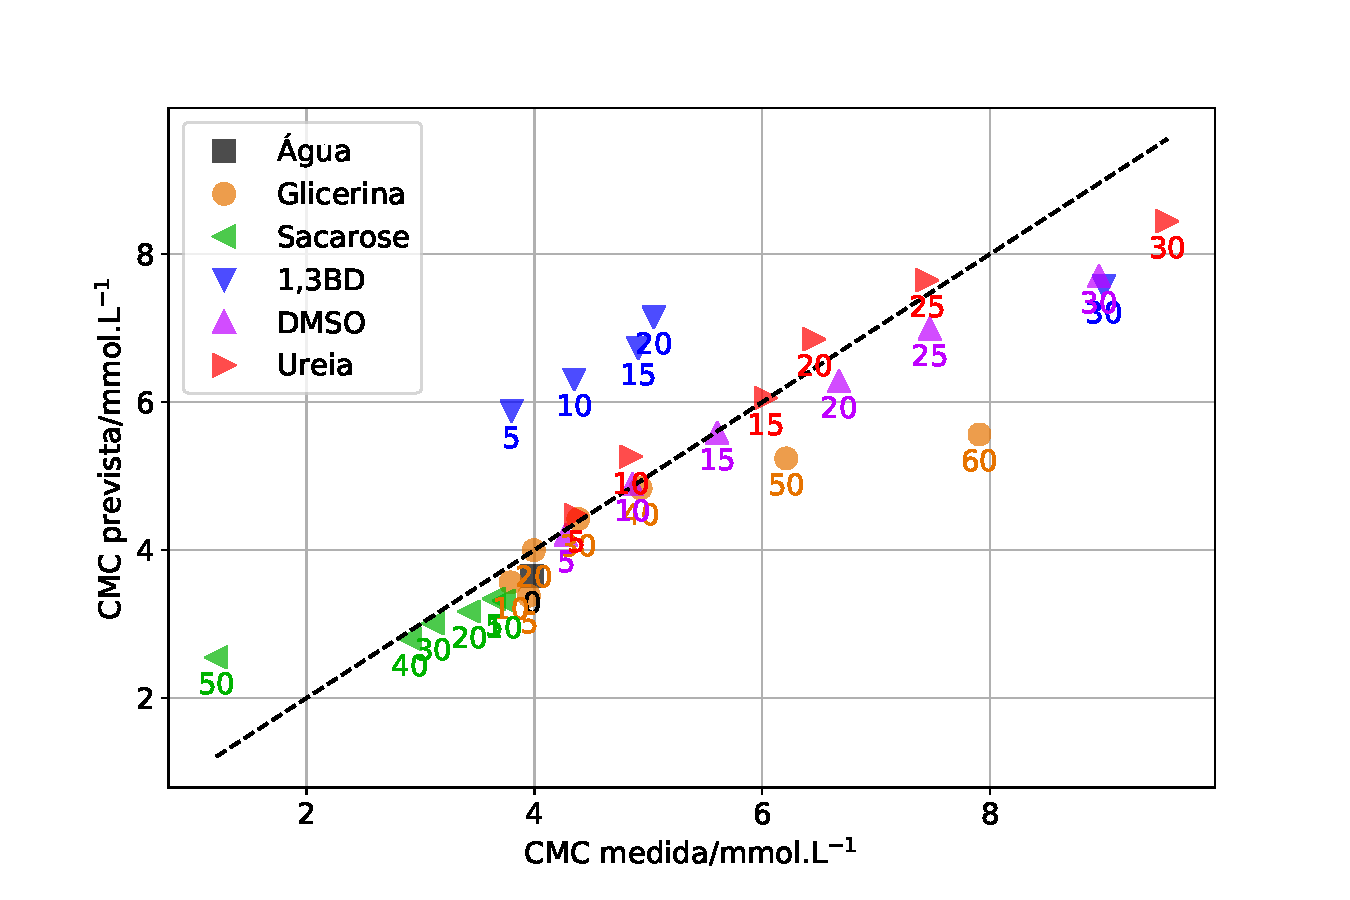
\includegraphics[width=0.7\textwidth]{imagens/itc/PLS_cmc_pirouette}
			\caption{Comportamento do modelo de \cmc{} criado, mostrando a correlação entre os valores observados e previstos. A reta preta tracejada o modelo perfeito, onde há uma relação 1:1 entre o observado e o previsto. A reta vermelha mostra o modelo criado.}
			\label{fig:pls_cmc_pirouette}
		\end{figure}
	
%		\begin{figure}[h]
%			\centering
%			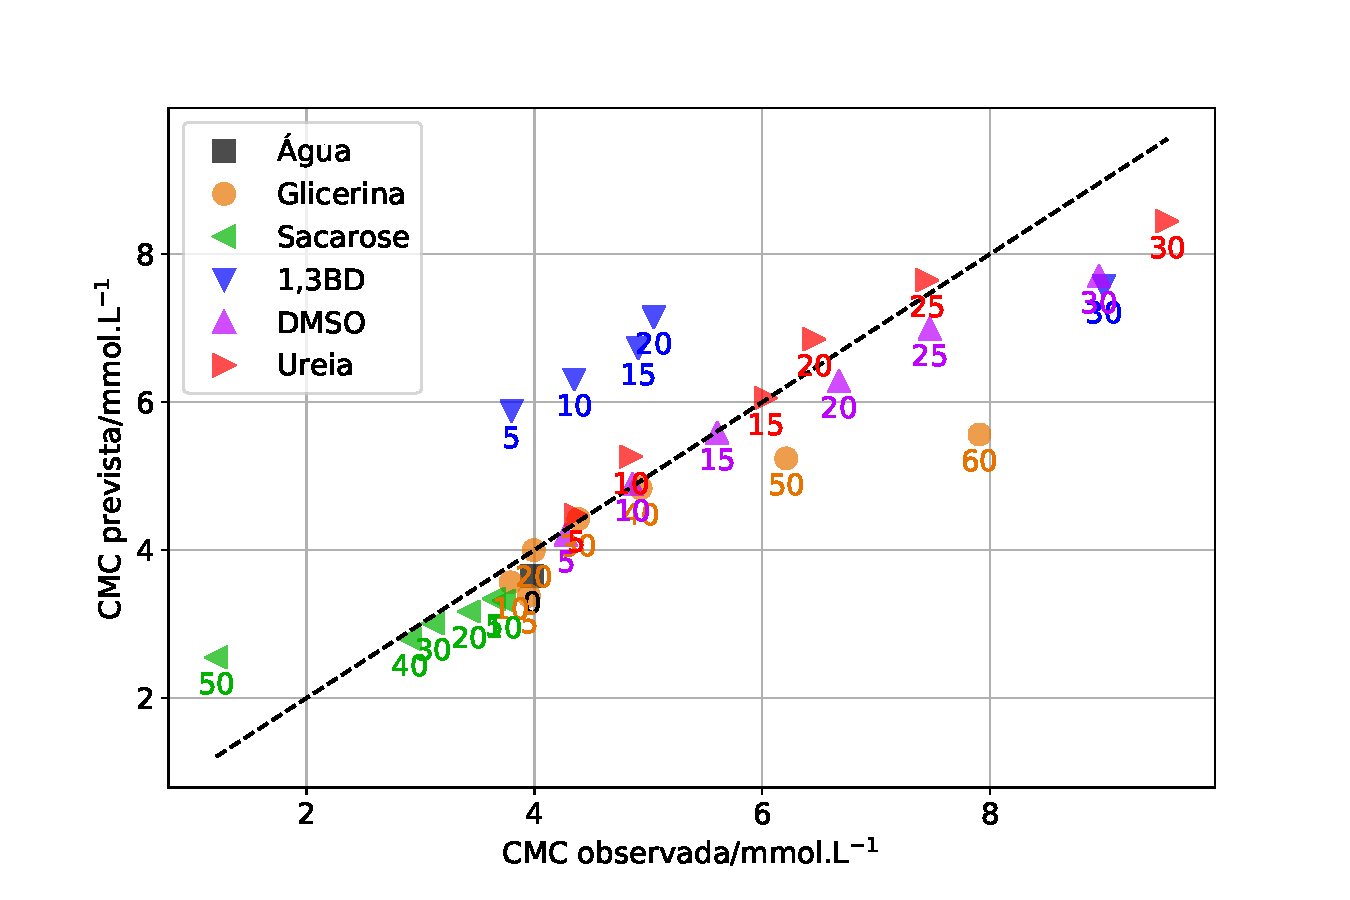
\includegraphics[width=0.7\textwidth]{imagens/itc/PLS_cmc_python}
%			\caption{}
%			\label{fig:pls_cmc_python}
%		\end{figure}  
	
		\begin{figure}[H]
			\centering
			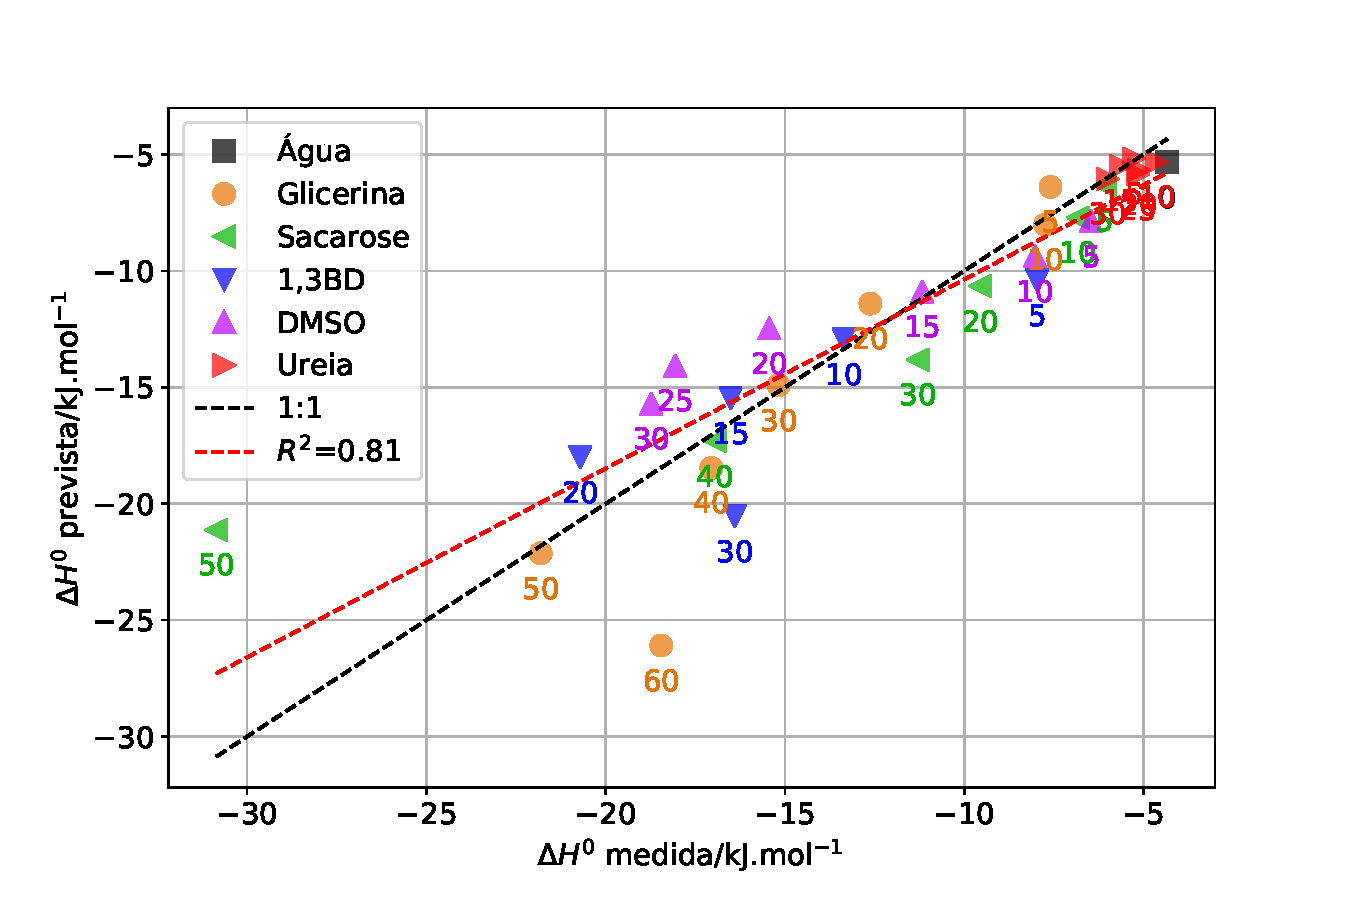
\includegraphics[width=0.7\textwidth]{imagens/itc/PLS_dh_pirouette}
			\caption{Comportamento do modelo de \DHmic{} criado, mostrando a correlação entre os valores observados e previstos. A reta preta tracejada o modelo perfeito, onde há uma relação 1:1 entre o observado e o previsto. A reta vermelha mostra o modelo criado, junto com a qualidade do ajuste.}
			\label{fig:pls_dh_pirouette}
		\end{figure} 
	
%		\begin{figure}[h]
%			\centering
%			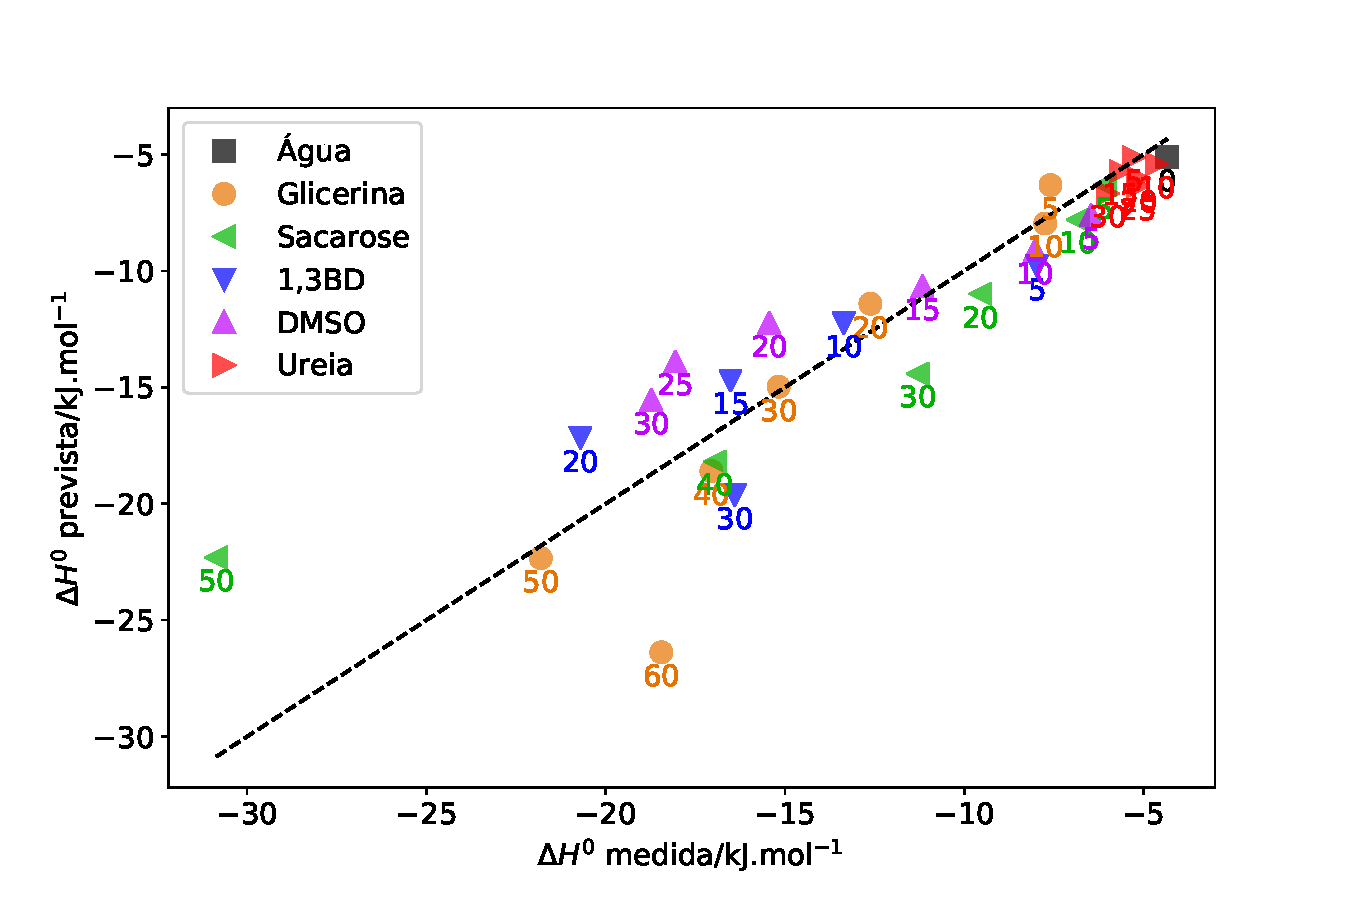
\includegraphics[width=0.7\textwidth]{imagens/itc/PLS_dh_python}
%			\caption{}
%			\label{fig:pls_dh_python}
%		\end{figure} 
		
		O código para fazer análise de PLS em Python, e uma figura semelhante à figura \ref{fig:pls_cmc_pirouette} está na listagem \ref{lst:pls_cmc_python}.
		
		\begin{listing}[h]
			\inputminted{python}{./python/pls_cmc_sklearn.py}
			\caption{Código utilizado para gerar a dependência de \cmc{} com os parâmetros estudados, resultando na Fig. \ref{fig:pls_cmc_pirouette}. A tabela de dados utilizada possui em cada linha as misturas utilizadas, suas concentrações em \% m/m, as variáveis dependentes (\cmc{} e \DHmic) e as variáveis independentes (\(n\), \(\varepsilon\), \(G\))}
			\label{lst:pls_cmc_python}
		\end{listing}
		
		O resultado desse modelo é um conjunto de coeficientes que, quando multiplicados pelos parâmetros escolhidos (\(n\), \(\varepsilon\), \(G\)), resultam em alguma das propriedades (\cmc, \DHmic). O vetor fornecido não possui unidades pois os dados foram autoescalados, então é necessário desfazer o autoescalamento para obter uma equação que utiliza coeficientes com as unidades utilizadas neste trabalho. As equações \ref{eqn:PLS_cmcs} e \ref{eqn:PLS_dhs} possuem tanto as relações em unidades usuais (a) quanto autoescaladas (b) para a \cmc{} e \DHmic, respectivamente.
				
		\begin{subequations}
			\begin{align}
				\textrm{CMC}               & = -7,206G              + 0,225\varepsilon             + 27,955n -31,871  \label{eqn:PLS_cmc}     \\
				\textrm{CMC}_{\textrm{AS}} & = -0,941G_\textrm{AS}  + 0,864\varepsilon_\textrm{AS} +0,319n_\textrm{AS} \label{eqn:PLS_cmc_AS}
			\end{align}
			\label{eqn:PLS_cmcs}
		\end{subequations}
		
		\begin{subequations}
			\begin{align}
				\Delta H_\textrm{mic}^0 &= 7,64G + 0,395\varepsilon-119n+101  \label{eqn:PLS_dh} \\
				\Delta H_\textrm{mic, AS}^0 &= 0,300G_\textrm{AS} + 0,458\varepsilon_\textrm{AS} - 0,414n_\textrm{AS}  \label{eqn:PLS_dh_AS}
			\end{align}
			\label{eqn:PLS_dhs}
		\end{subequations}
		
		\FloatBarrier
		\subsection{OLS}
		
		Outra metodologia que pode ser utilizada para realizar essas correlações é a dos mínimos quadrados ordinários (\emph{ordinary least squares}, OLS). Esse método é mais simples do que o PLS. Neste caso, o ajuste é feito reduzindo-se os mínimos quadrados da equação \ref{eqn:ols_modelo_cmc}.
		
		\begin{equation}
			\textrm{CMC} = a_G \cdot G + a_\varepsilon \cdot \varepsilon + a_n \cdot n + e
			\label{eqn:ols_modelo_cmc}
		\end{equation}
		
		Esse tipo de ajuste é igual ao ajuste de uma equação linear, porém com mais de uma variável independente. Foram feitos ajustes por mínimos quadrados ordinários tanto para a previsão da \cmc{} quanto a \DHmic. Os resultados dos ajustes estão nas figuras \ref{fig:ols_cmc_python} e \ref{fig:ols_dh_python}.
		
		\begin{figure}[h]
			\centering
			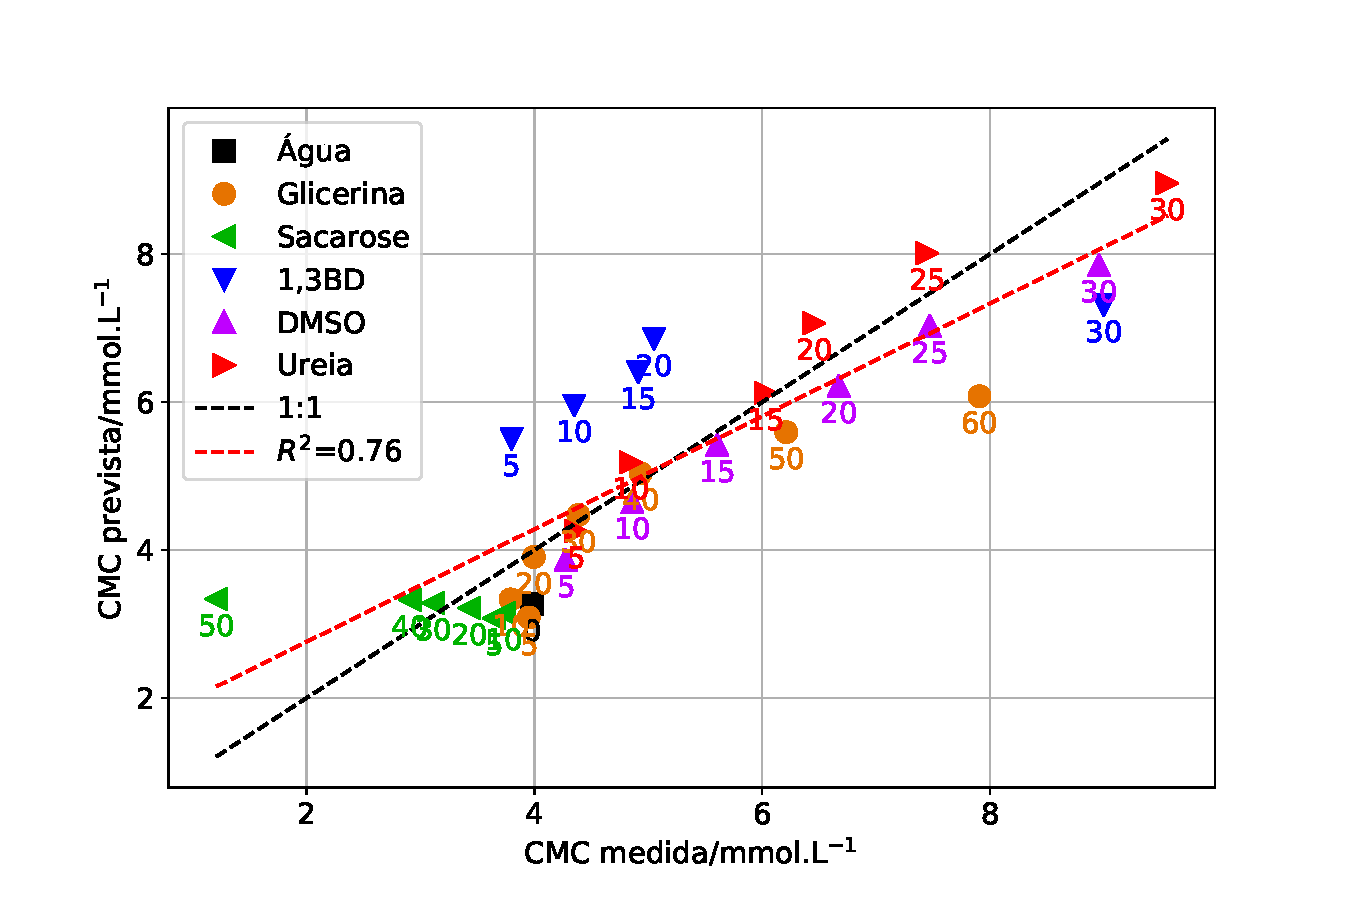
\includegraphics[width=0.7\textwidth]{imagens/itc/ols_cmc_python}
			\caption{}
			\label{fig:ols_cmc_python}
		\end{figure}
		
		\begin{figure}[h]
			\centering
			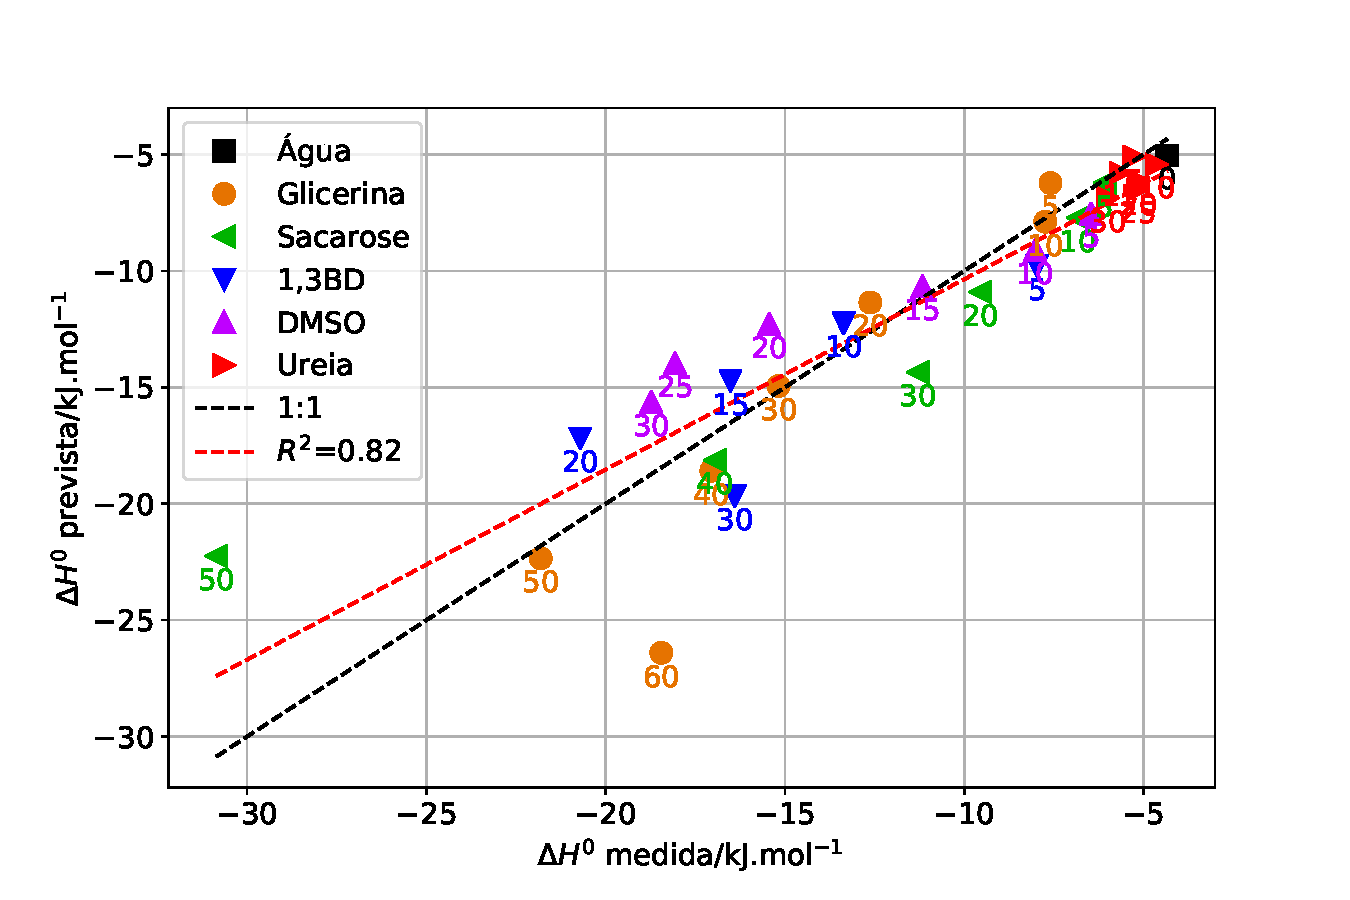
\includegraphics[width=0.7\textwidth]{imagens/itc/ols_dh_python}
			\caption{}
			\label{fig:ols_dh_python}
		\end{figure}
		
		Para realizar as análises e criar a figura \ref{fig:ols_cmc_python}, utilizou-se o código \ref{lst:ols_cmc_python}.
		
		\begin{listing}[h]
			\inputminted{python}{./python/ols_cmc_statsmodels.py}
			\caption{Código utilizado para gerar a dependência de \cmc{} com os parâmetros estudados, resultando na Fig. \ref{fig:ols_cmc_python}. A tabela de dados utilizada possui em cada linha as misturas utilizadas, suas concentrações em \% m/m, as variáveis dependentes (\cmc{} e \DHmic) e as variáveis independentes (\(n\), \(\varepsilon\), \(G\)).}
			\label{lst:ols_cmc_python}
		\end{listing}
		
		Os modelos obtidos estão nas equações \ref{eqn:ols_cmcs} e \ref{eqn:ols_dhs}. O pacote fornece os parâmetros autoescalados. Para convertê-los em parâmetros nas unidades tradicionais, é necessário desescalá-los, o que foi feito com o código da listagem \ref{lst:ols_cmc_conversao}.
		
		\begin{subequations}
			\begin{align}
			\textrm{CMC}               & = -7,073G              + 0,239\varepsilon             + 43,5n              -54,67  \label{eqn:ols_cmc}     \\
			\textrm{CMC}_{\textrm{AS}} & = -0,917G_\textrm{AS}  + 0,919\varepsilon_\textrm{AS} +0,497n_\textrm{AS}          \label{eqn:ols_cmc_AS}
			\end{align}
			\label{eqn:ols_cmcs}
		\end{subequations}
		
		\begin{subequations}
			\begin{align}
			\Delta H_\textrm{mic}^0     &= 6,29G              + 0,372\varepsilon             - 138n               + 132  \label{eqn:ols_dh} \\
			\Delta H_\textrm{mic, AS}^0 &= 0,258G_\textrm{AS} + 0,432\varepsilon_\textrm{AS} - 0,480n_\textrm{AS}        \label{eqn:ols_dh_AS}
			\end{align}
			\label{eqn:ols_dhs}
		\end{subequations}
		
		\begin{listing}[h]
			\inputminted{python}{./python/ols_cmc_conversão.py}
			\caption{Código utilizado para transformar os parâmetros dos ajustes de autoescalados para valores habituais.}
			\label{lst:ols_cmc_conversao}
		\end{listing}
		
		\FloatBarrier
		\section{Decomposição em propriedades fundamentais}
		TODO
		

		
		
